\documentclass[12pt,a4paper]{article}
\usepackage{amsmath, amssymb, amsthm}
\usepackage{graphicx}
\usepackage{subcaption}   % Required for subfigures
\usepackage{geometry}
\usepackage{caption}
\usepackage{float}
\usepackage{hyperref}
\usepackage{enumitem}
\usepackage{mathtools}
\usepackage{physics}
\usepackage{booktabs}
\usepackage{multirow}
\usepackage{tabularx}
\usepackage{marvosym}
\usepackage{algorithm}
\usepackage{algpseudocode}

\geometry{margin=1in}
\hypersetup{
    colorlinks=true,
    linkcolor=blue,
    urlcolor=blue,
    pdftitle={Bachelor Thesis},
    pdfauthor={}
}


\title{Bachelor Thesis}
\author{Viktor Tevosyan}
\date{}

% Definitions
\begin{document}
\newtheorem{definition}{Definition}
\newtheorem{theorem}{Theorem}
\newtheorem{lemma}{Lemma}

\newcommand{\thesistitle}{Neural Network-Based Optimization in FBP for
Computed Tomography}
\newcommand{\firstsupervisor}{Prof. Dr. Anne Wald}
\newcommand{\secondsupervisor}{Prof. Dr. Alexander Ecker}
\newcommand{\authorname}{Viktor Tevosyan}
\newcommand{\university}{Georg-August-Universität Göttingen}
\newcommand{\department}{Institute of Computer Science}
\newcommand{\thesistype}{Bachelor's Thesis} % Bachelor's Thesis or Master's Thesis
\newcommand{\course}{Applied Computer Science}
\newcommand{\matrikelnumber}{29826385}
\newcommand{\keywords}{Put keywords here} % Set keywords that describe your report
\newcommand{\documentlanguage}{de-DE} % Required for PDF/A
\newcommand{\submissiondate}{\today}

\begin{titlepage}

\includegraphics[width=6.5cm]{Bachelorthesis/logo-goettingen.pdf} 
	
\begin{center}
	
	\vspace*{.06\textheight}
	{\LARGE \textbf{\thesistype}\\}
	submitted in partial fulfillment of the\\
	requirements for the course ``\course''\\[0.5cm]
	
	
	\rule{.9\linewidth}{.6pt} \\[0.4cm] % Horizontal line
	{\huge \bfseries \thesistitle}\vspace{0.4cm}
	\rule{.9\linewidth}{.6pt} \\[1.5cm] % Horizontal line
	
	\Large\authorname\\
	\hfill\\
	\large MatrNr: \matrikelnumber\\ \vfill
	\begin{tabular}{@{}ll}
		First Supervisor: &\firstsupervisor\\
		Second Supervisor: &\secondsupervisor
	\end{tabular}
	\vfill
	\university\\
	\department\\
	ISSN: 1612-6793
	\vfill
	{\large \submissiondate}\\[4cm] % Date
	
	\vfill
\end{center}

\newpage
\vfill

% Then we have the contact


{
\null
\flushleft
\normalsize
\vspace{14cm}

Georg-August-Universit\"at G\"ottingen\\
Institute of Computer Science\\[3ex]
Goldschmidtstra\ss{}e 7\\
37077 G\"ottingen\\
Germany\\[3ex]

\begin{tabular}{@{}ll}
  \Telefon & +49 (551) 39-172000\\
  \fax & +49 (551) 39-14403\\
  \Letter & \href{mailto:office@informatik.uni-goettingen.de}{office@informatik.uni-goettingen.de}\\
  \Mundus & \url{www.informatik.uni-goettingen.de}
\end{tabular}
}



\end{titlepage}
\tableofcontents
\newpage

\section{Motivation}

Computed Tomography is a medical imaging technique introduced in the 1970s, used to obtain detailed internal images of the body. CT has become an essential tool to supplement conventional X-ray imaging, enabling the creation of 3D images by combining 2D slices of the body's interior. By providing more precise and detailed images than X-rays, CT scans can help diagnose muscle and bone conditions (e.g., fractures), locate tumors, infections, or blood clots, and detect internal injuries or bleeding after trauma.
\newline\newline
The process of reconstructing a single CT slice from raw measurements is non-trivial and can be formulated as an inverse problem. Today, several algorithms are used to reconstruct internal body slices from CT scan measurements, represented as sinograms. The Filtered Backprojection (FBP) algorithm reconstructs a 2D image slice from a set of 1D projections by first filtering and then back-projecting them. FBP provides a closed-form, analytical solution to the inverse problem and is computationally efficient. However, the quality of its results depends heavily on the sinogram data and, consequently, on the radiation dose used in the scan. While high-dose CT scans produce sharp, high-quality reconstructions, they expose patients to harmful radiation. Reducing the dose increases noise, degrading image sharpness and potentially compromising diagnosis.
\newline\newline
To address the challenge of high noise in low-dose CT images, deep learning offers a powerful solution due to its ability to learn complex patterns and relationships between noisy and noise-free images. Once trained, such models can effectively denoise unseen images. One possible approach is to post-process the FBP-reconstructed image with a neural network, as demonstrated in prior work. However, this post-processing method operates solely on the reconstructed image and does not utilize the raw CT measurements, which may limit its learning potential.
\newline\newline
This raises the question: Would it be beneficial for the reconstruction quality, if we integrate a neural network earlier in the pipeline and include the sinogram information into the objective function? Would such integration also improve the post-processing step?
\newpage
\section{Basics}

\subsection{What is a CT scan?}
\label{what_is_ct}

Computed tomography (CT) is a diagnostic imaging method that uses X-rays to generate detailed cross-sectional images of the human body~\cite{nibib_ct}. X-rays are a form of electromagnetic radiation with higher energy than visible light and the ability to penetrate different types of matter, as shown in Figure~\ref{fig1} \cite{nibib_xray}. 

\begin{figure}[H]
    \centering
    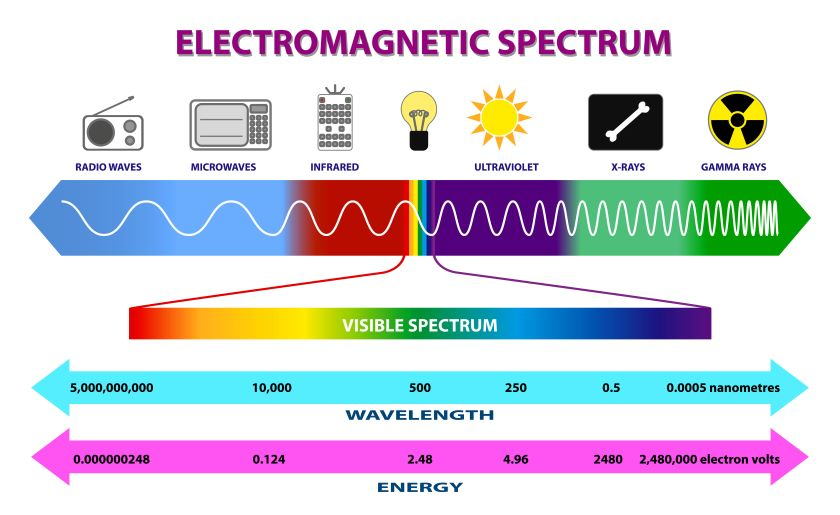
\includegraphics[width=0.4\textwidth]{Bachelorthesis/UsedImages/fig1.jpg}
    \caption{The electromagnetic spectrum \cite{nibib_xray}}
    \label{fig1}
\end{figure}

The absorption of X-rays depends mainly on the density and atomic number of the tissue they pass through. Dense structures such as bone, which contain calcium, absorb more radiation than soft tissues. This explains why bones appear brighter on radiographs and CT images \cite{nibib_xray}. 

A CT scanner consists of a rotating X-ray tube and a detector system housed within a circular structure known as the \textit{gantry}, shown in Figure~\ref{fig2}. During scanning, the patient lies on a motorized table that slowly moves through the gantry. The X-ray tube rotates around the body, while detectors measure how much radiation passes through the tissues. These measurements are collected from many angles \cite{nibib_ct}. 


\begin{figure}[h!]
    \centering
    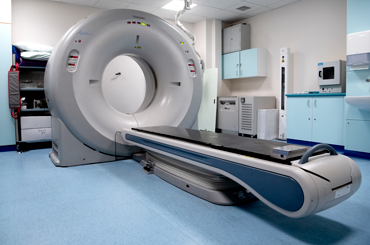
\includegraphics[width=0.5\linewidth]{Bachelorthesis//UsedImages/fig2.png}
    \caption{A CT scanner~\cite{cancerresearchuk_ctscan_fig}}
    \label{fig2}
\end{figure}

Once sufficient data from a full rotation is collected, the computer applies reconstruction algorithms to create a two-dimensional image slice. By repeating this process while the table advances, multiple slices are acquired. These slices can be viewed individually or combined into a three-dimensional model, providing a comprehensive view of the patient’s anatomy \cite{nibib_ct}.



\subsection{CT Scan Acquisition Modes}
\label{ct_scan_modes}

CT scanning can be performed using different acquisition modes, each with distinct characteristics.
\newline\newline
\textbf{Sequential (axial) scanning} was the first method developed. In this mode, the X-ray source and detector rotate around the patient to acquire a single slice of data, called a "slab". Once the slice is reconstructed, the patient table moves to the next position for the following axial scan, as illustrated in Figure~\ref{fig3}. For example, to cover 160\,mm in the longitudinal direction with 10\,mm slabs, 16 rotations are required. The main limitation of sequential scanning is patient motion between scans, which can lead to misalignment and artifacts in the reconstructed 3D volume. This is exacerbated by the acceleration and deceleration of the table and the relatively long total scan time needed to cover the area of interest \cite{nett2019ctscanmodes}.
\newline\newline
\textbf{Helical (spiral) scanning} addresses these limitations by continuously moving the patient table while the X-ray source rotates around the patient. This results in a helical path of the X-ray beam through the body, allowing for faster acquisition and reducing the risk of motion artifacts, as shown in Figure~\ref{fig3}. Helical scanning also provides continuous data collection, enabling flexible image reconstruction from any position along the scanned volume \cite{nett2019ctscanmodes}.

\begin{figure}[H]
    \centering
    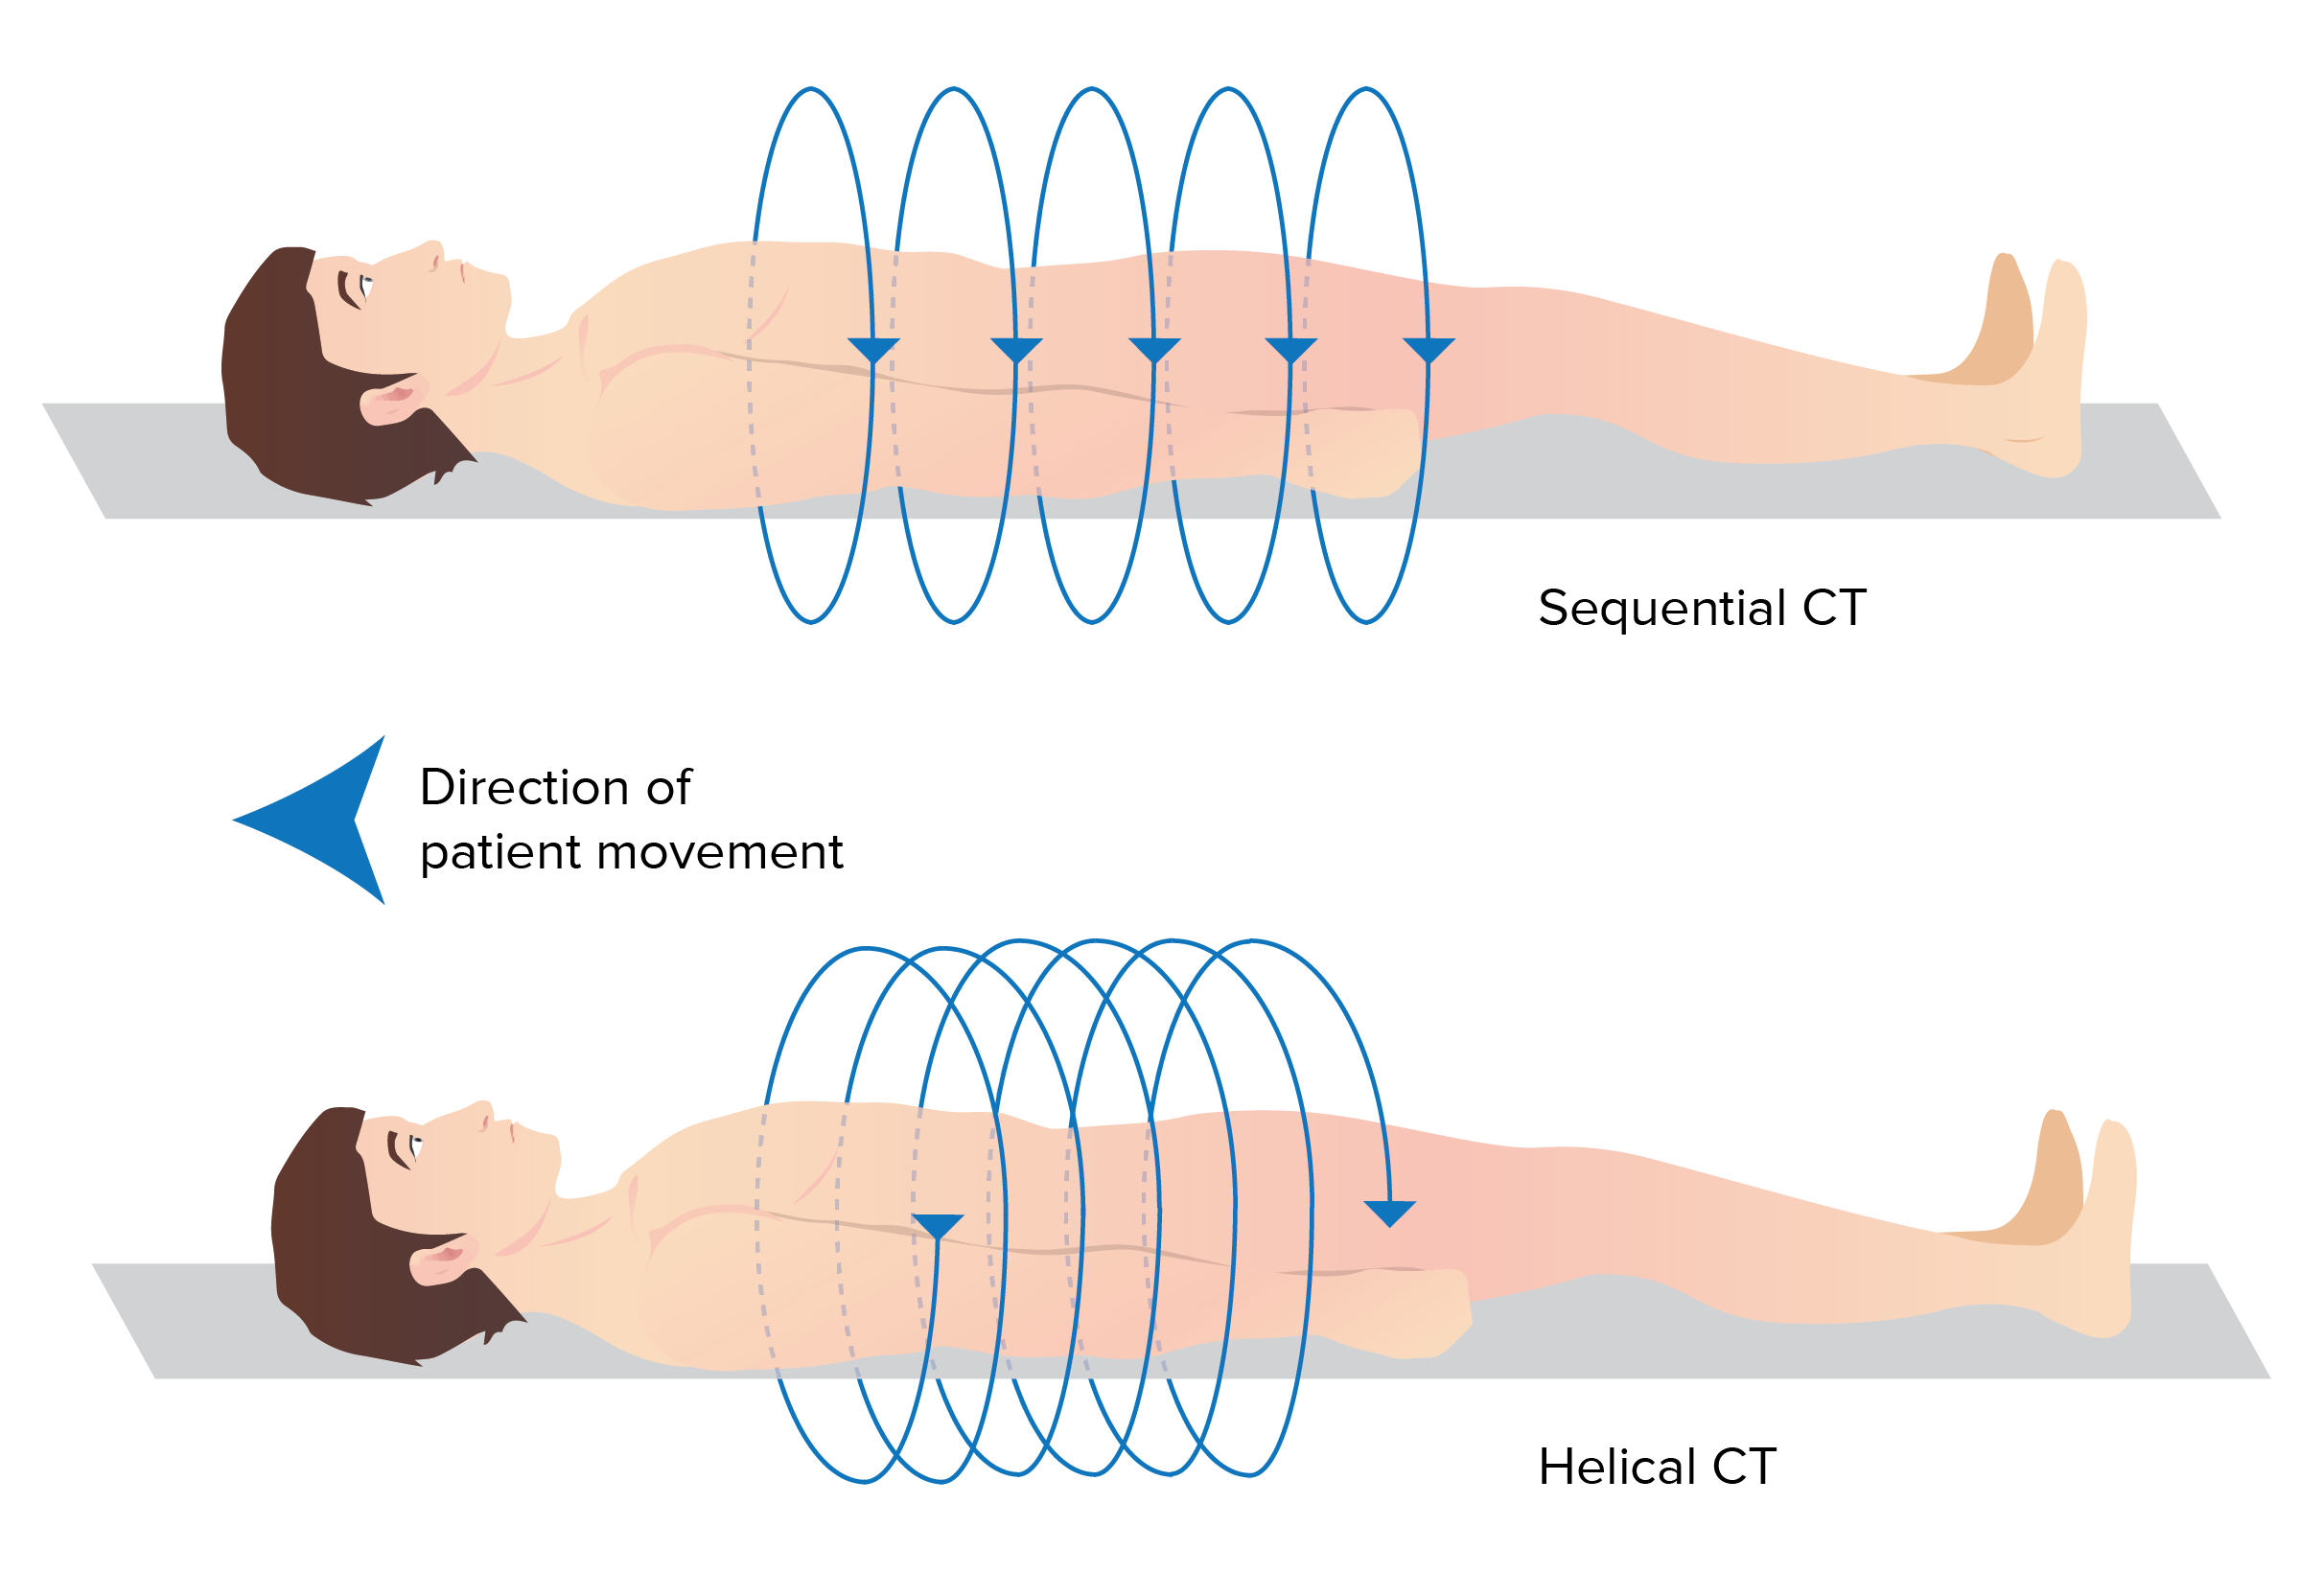
\includegraphics[width=0.8\textwidth]{Bachelorthesis/UsedImages/fig3.png}
    \caption{Illustration of sequential (axial) and helical (spiral) CT scanning~\cite{lecturio_ct_2025}}
    \label{fig3}
\end{figure}


\subsection{Quick Insight into CT Scan Geometries}
\label{ct_scan_geometries}

CT scanners use different X-ray beam geometries to cover the patient’s body during imaging. The most common geometries are parallel-beam, fan-beam, and cone-beam arrangements \cite{nett2019ctgenerations}.

\paragraph{Parallel-beam geometry}
In this setup, X-rays are assumed to be perfectly parallel as they pass through the tissue and reach the detectors, as illustrated in Figure~\ref{fig5}. The source and detector array rotate around the patient to capture measurements from multiple angles and offsets.

\paragraph{Fan-beam geometry}
The X-rays are emitted in a fan-shaped pattern. A single source directs beams toward the patient, and a curved detector array captures the transmitted X-rays. The source-detector pair advances to acquire the next projection after each rotation, as shown in Figure~\ref{fig5}. This geometry allows faster scanning because complete 360° rotations are not required for each slice.

\paragraph{Cone-beam geometry}
Extending the fan-beam concept to three dimensions, the X-ray source emits a cone-shaped beam that covers a volumetric region of the patient. This enables the acquisition of 3D data in a single rotation, reducing the number of table movements needed to cover the area of interest (Figure~\ref{fig5}) \cite{nett2019ctgenerations}.

\begin{figure}[H]
    \centering
    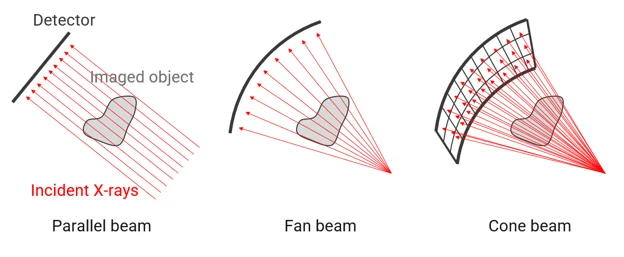
\includegraphics[width=0.7\textwidth]{Bachelorthesis/UsedImages/fig5.png}
    \caption{Visualization of different CT scan geometries}
    \label{fig5}
\end{figure}

\subsection{Mathematical formulation of parallel-beam CT}
\label{Formulation}

The goal of computed tomography (CT) is to reconstruct an image of the inside of the human body from measurements of X-ray attenuation. In practice, the scanner only records the change in X-ray intensity along many straight lines that pass through the body. Our task is to express this as a mathematical problem: what exactly is measured, and how can we recover the unknown attenuation coefficients?
\newline\newline
To make this precise, we restrict ourselves to a single two-dimensional axial slice, modeled with parallel-beam geometry. In this setting, the object under investigation is represented by a bounded domain $\Omega \subset \mathbb{R}^2$, and the function
\[
f : \mathbb{R}^2 \to \mathbb{R}
\]
denotes the X-ray attenuation coefficients. Since $f$ vanishes outside the object, we may assume that $\mathrm{supp}(f) \subset \Omega$~\cite{math_of_ct}. For completeness, we recall two basic definitions that will be used throughout this section.

\begin{definition}[Convex set]
A set $\Omega \subset \mathbb{R}^2$ is called \emph{convex} if for all $x,y \in \Omega$ the line segment between them lies in $\Omega$, i.e.
\[
\forall t \in [0,1]: \quad (1-t)x + ty \in \Omega.
\]
\end{definition}

\begin{definition}[Support of a function]
Let $f : X \to \mathbb{R}$. The \emph{support} of $f$ is the set
\[
\mathrm{supp}(f) := \{ x \in X : f(x) \neq 0 \}.
\]
\end{definition}

---

\paragraph{Modeling X-ray paths.}
An individual X-ray travels along a straight line through $\Omega$. We parametrize lines using an angle $\theta \in [0,\pi)$ and an offset $s \in \mathbb{R}$. To this end we introduce the unit vectors
\[
\Theta_\theta := \begin{pmatrix} \cos \theta \\ \sin \theta \end{pmatrix},
\qquad
\Theta_\theta^\perp := \begin{pmatrix} -\sin \theta \\ \cos \theta \end{pmatrix}.
\]
Then the line $L(\theta,s)$ can be written as
\begin{equation}
L(\theta,s) = \{ \gamma_{\theta,s}(t) : t \in \mathbb{R} \},
\qquad
\gamma_{\theta,s}(t) := s \Theta_\theta + t \Theta_\theta^\perp.
\label{eq:line_param}
\end{equation}

---

\paragraph{Beer's law.}
Let $I(x)$ denote the X-ray intensity at a point $x \in \mathbb{R}^2$. Along a line $\gamma(t)$, the intensity decreases due to absorption. Beer's law states that the loss of intensity over a small interval $\Delta t$ is proportional to both the current intensity and the attenuation coefficient:
\[
I(\gamma(t+\Delta t)) - I(\gamma(t)) \approx -f(\gamma(t))\,I(\gamma(t))\,\Delta t.
\]
Passing to the limit $\Delta t \to 0$, we obtain the differential equation
\begin{equation}
\frac{\mathrm{d}}{\mathrm{d}t}(I\circ \gamma)(t) = -f(\gamma(t))(I\circ \gamma)(t).
\label{eq:beer}
\end{equation}
Dividing both sides by $(I\circ \gamma)(t)$ shows that
\begin{equation}
\frac{\mathrm{d}}{\mathrm{d}t} \ln\bigl((I\circ \gamma)(t)\bigr) = -f(\gamma(t)).
\label{eq:beer_log}
\end{equation}
Integrating \eqref{eq:beer_log} from $t_0$ (source position $x_0$) to $t_1$ (detector position $x_1$) yields
\begin{equation}
\ln\!\left(\frac{I(\gamma(t_1))}{I(\gamma(t_0))}\right) 
= -\int_{t_0}^{t_1} f(\gamma(s)) \,\mathrm{d}s.
\label{eq:line_integral}
\end{equation}
Thus, the logarithm of the intensity ratio encodes exactly the line integral of $f$ along the path of the ray~\cite{math_of_ct_wald}.

---

\paragraph{Radon transform.}
Equation \eqref{eq:line_integral} motivates a mathematical operation that collects all such line integrals of $f$.

\begin{definition}[Radon transform]
For $f \in L^1(\mathbb{R}^2)$, the \emph{Radon transform} is
\begin{equation}
(\mathcal{R}f)(\theta,s) := \int_{\mathbb{R}} f(s \Theta_\theta + t \Theta_\theta^\perp)\, \mathrm{d}t,
\label{eq:radon}
\end{equation}
where $(\theta,s) \in [0,\pi)\times \mathbb{R}$.
\end{definition}
The Radon transform maps a two-dimensional function into its line integrals along all possible straight lines. In CT, the measured sinogram data is precisely $(\mathcal{R}f)(\theta,s)$.

---

\paragraph{Fourier analysis.}
To reconstruct $f$ from its Radon transform, we exploit the connection to the Fourier transform.

\begin{definition}[Fourier transform]
Let $f \in L^1(\mathbb{R}^d)$. Its \emph{Fourier transform} is defined by
\begin{equation}
(\mathcal{F}f)(\xi) := \int_{\mathbb{R}^d} f(x)\,e^{-i x^T \xi}\, \mathrm{d}x,
\label{eq:fourier}
\end{equation}
and its inverse by
\begin{equation}
f(x) = \frac{1}{(2\pi)^d}\int_{\mathbb{R}^d} (\mathcal{F}f)(\xi)\,e^{i \xi^T x}\, \mathrm{d}\xi.
\label{eq:fourier_inverse}
\end{equation}
\end{definition}

If $g:[0,\pi)\times \mathbb{R} \to \mathbb{R}$, we denote by $\mathcal{F}_2 g$ the Fourier transform of $g$ in the second variable, i.e.
\[
(\mathcal{F}_2 g)(\theta,\xi) := \int_{\mathbb{R}} g(\theta,s)\, e^{-i s \xi}\,\mathrm{d}s.
\]

---

\paragraph{Fourier slice theorem.}
The following classical result is fundamental for CT reconstruction \cite{math_of_ct}.

\begin{theorem}[Fourier slice theorem]
\label{thm:fourier_slice}
Let $f \in L^1(\mathbb{R}^2)$. Then
\begin{equation}
(\mathcal{F}f)(\Theta_\theta \xi) = (\mathcal{F}_2 \mathcal{R}f)(\theta,\xi),
\qquad (\theta,\xi) \in [0,\pi)\times\mathbb{R}.
\label{eq:fourier_slice}
\end{equation}
\end{theorem}

\begin{proof}
Starting from the right-hand side,
\[
(\mathcal{F}_2 \mathcal{R}f)(\theta,\xi) 
= \int_{\mathbb{R}} \biggl[ \int_{\mathbb{R}} f(s \Theta_\theta + t \Theta_\theta^\perp)\,\mathrm{d}t \biggr] e^{-i s \xi}\,\mathrm{d}s.
\]
By Fubini’s theorem, this equals
\[
\int_{\mathbb{R}^2} f(s\Theta_\theta + t\Theta_\theta^\perp)\, e^{-i s \xi}\, \mathrm{d}(s,t).
\]
The substitution $x = s\Theta_\theta + t\Theta_\theta^\perp$ has Jacobian determinant $1$, hence
\[
\int_{\mathbb{R}^2} f(x)\, e^{-i x^T(\Theta_\theta \xi)}\, \mathrm{d}x = (\mathcal{F}f)(\Theta_\theta \xi).
\]
\end{proof}

The Fourier slice theorem \eqref{eq:fourier_slice} shows that the one-dimensional Fourier transform of a projection at angle $\theta$ is equal to a central line in the two-dimensional Fourier transform of $f$. This identity is the cornerstone of the filtered back-projection algorithm.

---

\paragraph{Discretization.}
For practical computation, continuous transforms are replaced by discrete analogues. We recall the discrete Fourier transform (DFT) and Riemann sums, which form the numerical foundation of reconstruction algorithms.

\begin{definition}[Discrete Fourier transform~\cite{Osgood_Fourier}]
\label{def:DFT}
Let $\mathbf{x} = (x_0,\dots,x_{N-1}) \in \mathbb{C}^N$. Its DFT is
\begin{equation}
X_k = \sum_{n=0}^{N-1} x_n e^{-i \tfrac{2\pi k}{N}n}, \qquad k=0,\dots,N-1.
\label{eq:dft}
\end{equation}
The inverse DFT is
\begin{equation}
x_n = \frac{1}{N}\sum_{k=0}^{N-1} X_k e^{i \tfrac{2\pi k}{N}n}, \qquad n=0,\dots,N-1.
\label{eq:idft}
\end{equation}
\end{definition}

\begin{definition}[Riemann sum~\cite{SFU_RiemannSums}]
Let $f:[a,b]\to \mathbb{R}$ and let $P=(x_1,\dots,x_{N+1})$ be a partition with $a=x_1<\dots<x_{N+1}=b$. A \emph{Riemann sum} of $f$ with respect to $P$ is
\begin{equation}
S_P(f) := \sum_{i=1}^N f(x_i^*)\,\Delta x_i,
\qquad \Delta x_i = x_{i+1}-x_i,\ x_i^*\in[x_i,x_{i+1}).
\label{eq:riemann}
\end{equation}
\end{definition}

\subsection{Expression of the problem}
\label{problem_expr}

In Section~\ref{Formulation}, we introduced the Radon transform as the operator that connects the physics of X-ray attenuation with the mathematics of integral geometry. Our goal is now to cast the reconstruction task as an inverse problem in a precise functional-analytic setting, and to investigate its properties. This will allow us to understand both the strengths and the limitations of the Radon transform as a forward model for computed tomography (CT).
\newline\newline
The function of interest is  
\[
f : \mathbb{R}^2 \to \mathbb{R},
\]  
which describes the X-ray absorption coefficient of the patient in a given slice. As argued before, $f$ is only relevant inside the scanned region. It is therefore natural to assume that $f$ has bounded, convex support $\Omega \subset \mathbb{R}^2$. Without loss of generality, we may place $\Omega$ inside a disk of radius $R > 0$ centered at the origin,  
\[
\Omega \subset \overline{\mathcal B_R (0)}.
\]  
This motivates the definition of the restricted $L^2$ space  
\[
L^2_{R} := \{ f \in L^2(\mathbb R^2) : \mathrm{supp}(f) \subseteq \overline{\mathcal B_R (0)} \},
\]  
and consequently, we will always assume  
\[
f \in L^2_R \subset L^2(\mathbb R^2).
\]  
The Hilbert space structure of $L^2$ provides the natural inner product  
\[
\langle f, h \rangle_{L^2(\mathbb R^2)} := \int_{\mathbb R^2} f(x) \overline{h(x)} \,\mathrm{d}x,
\]  
which will later allow us to formulate reconstruction methods using adjoint operators and variational principles.
\newline\newline
Within this setting, the Radon transform acts as a linear operator  
\[
\mathcal{R} : L^2(\mathbb R^2) \to L^2([0,\pi) \times \mathbb R),
\]  
mapping the absorption coefficient $f$ to its sinogram $g$, i.e. the collection of line integrals:  
\[
\mathcal{R} f = g.
\]  
The reconstruction problem is then naturally expressed as an inverse problem: recover $f$ from $g$.  In practice, measurements are noisy. If $g^\delta$ denotes the measured sinogram, then we assume an error model of the form  
\[
\norm{g - g^\delta} \leq \delta,
\]  
where $\delta > 0$ is the noise level. This noise sensitivity leads us to the concept of \emph{well-posedness}. In Hadamard’s sense, an inverse problem is only considered mathematically satisfactory if it admits a solution that is not only unique but also depends continuously on the data~\cite{math_of_ct_wald}.

\begin{definition}[Well-posedness~\cite{math_of_ct_wald}]
    \label{well-posed}
    Let $X,Y$ be Hilbert spaces. A linear inverse problem  
l    \[
        A f = g, \quad A : X \rightarrow Y, \quad \norm{g - g^\delta} \leq \delta,
    \]  
    is called \emph{well-posed} if:
    \begin{enumerate}
        \item (Existence) For each $g \in Y$, there exists $f \in X$ with $Af = g$.
        \item (Uniqueness) If $Af = A\tilde{f} = g$, then $f = \tilde{f}$.
        \item (Stability) The inverse operator $A^{-1}$ is continuous.
    \end{enumerate}
    If one of these properties fails, the problem is called \emph{ill-posed}.
\end{definition}


For the Radon transform, the uniqueness can be shown under our compact support assumption. The main difficulty lies in stability: the inverse of the Radon transform is not continuous, meaning that even small measurement errors $\delta$ can cause large reconstruction errors $\|f - f^\delta\|$. This instability is the central challenge in CT reconstruction.
\newline\newline
To prepare for reconstruction algorithms, we must first establish some operator-theoretic properties of the Radon transform. In particular, it is crucial to know whether $\mathcal{R}$ is bounded, injective, and what its adjoint operator $\mathcal{R}^*$ looks like. These aspects are captured in the following theorem.

\begin{theorem}
\label{inj+bound}
    The Radon transform  
    \[
    \mathcal{R} : L^2(\mathbb R^2) \to L^2([0, \pi) \times \mathbb{R})
    \]  
    is a linear operator, which is bounded and injective on $L^2_R$. Its adjoint  
    \[
    \mathcal{R}^* : L^2([0, \pi) \times \mathbb R) \to L^2(\mathbb R^2)
    \]  
    is given by  
    \[
        (\mathcal{R}^* g)(\mathbf{x}) = \int_0^\pi g(\theta,\mathbf{x}^T \Theta_\theta) \,\mathrm{d}\theta .
    \]
\end{theorem}

\begin{proof}
\emph{Linearity.}  
Linearity follows immediately from the properties of the Lebesgue integral. Indeed, for $f,h \in L^2_R$ and $\alpha, \beta \in \mathbb{R}$,  
\[
\mathcal{R}(\alpha f + \beta h)(\theta,s) 
= \int_\mathbb{R} \big( \alpha f(\gamma_{\theta,s}(t)) + \beta h(\gamma_{\theta,s}(t)) \big)\,\mathrm{d}t,
\]  
which can be rewritten as  
\[
\alpha \mathcal{R}f(\theta,s) + \beta \mathcal{R}h(\theta,s).
\]
\newline\newline
\emph{Boundedness.}  
To prove boundedness, we estimate the $L^2$-norm of $\mathcal{R} f$. For $f \in L^2_R$,  
\begin{align*}
\norm{\mathcal{R} f}_{L^2([0,\pi)\times \mathbb{R})}^2
&= \int_0^\pi \int_{-\infty}^\infty \big| \mathcal{R}f(\theta,s)\big|^2 \,\mathrm{d}s\,\mathrm{d}\theta \\
&= \int_0^\pi \int_{-R}^R \left| \int_{-\infty}^{+\infty} f(s\Theta_\theta + t \Theta_\theta^\perp)\,\mathrm{d}t \right|^2 \mathrm{d}s\,\mathrm{d}\theta .
\end{align*}
Applying Cauchy--Schwarz and extending the integration range yields
\[
\norm{\mathcal{R} f}_{L^2}^2
\leq 2R \int_0^\pi \int_{-\infty}^{+\infty} \int_{-\infty}^{+\infty} |f(s\Theta_\theta + t \Theta_\theta^\perp)|^2 \,\mathrm{d}t \,\mathrm{d}s \,\mathrm{d}\theta .
\]
For fixed $\theta$, consider the diffeomorphism
\[
\Phi_\theta : \mathbb{R}^2 \to \mathbb{R}^2, \quad (s,t) \mapsto s \Theta_\theta + t \Theta_\theta^\perp,
\]
whose Jacobian determinant satisfies $|\det(D\Phi_\theta)| = 1$. Hence,
\[
\norm{\mathcal{R} f}_{L^2}^2 \leq 2R \int_0^\pi \int_{\mathbb{R}^2} |f(\mathbf{x})|^2 \,\mathrm{d}\mathbf{x}\,\mathrm{d}\theta 
= 2\pi R \norm{f}_{L^2(\mathbb{R}^2)}^2 .
\]
Thus $\mathcal{R}$ is bounded with  
\[
\norm{\mathcal{R}}_{L^2_R \to L^2} \leq \sqrt{2\pi R}.
\]
\newline\newline
\emph{Adjoint operator.}  
Since $\mathcal{R}$ is bounded, an adjoint $\mathcal{R}^*$ exists. We compute explicitly:
\begin{align*}
\langle \mathcal{R} f, g \rangle_{L^2([0,\pi)\times \mathbb{R})}
&= \int_0^\pi \int_{-\infty}^\infty \mathcal{R}f(\theta,s) g(\theta,s)\,\mathrm{d}s\,\mathrm{d}\theta \\
&= \int_0^\pi \int_{-\infty}^\infty \int_{-\infty}^\infty f(\Phi_\theta(s,t)) g(\theta,s)\,\mathrm{d}t\,\mathrm{d}s\,\mathrm{d}\theta \\
&= \int_{\mathbb{R}^2} f(\mathbf{x}) \int_0^\pi g(\theta, \mathbf{x}^T \Theta_\theta)\,\mathrm{d}\theta \,\mathrm{d}\mathbf{x}.
\end{align*}
Hence, by definition of the adjoint,
\[
(\mathcal{R}^* g)(\mathbf{x}) = \int_0^\pi g(\theta, \mathbf{x}^T \Theta_\theta)\,\mathrm{d}\theta .
\]
\newline\newline
\emph{Injectivity.}  
Finally, to show injectivity on $L^2_R$, suppose $\mathcal{R} f = 0$. Then, by the Fourier slice theorem (Theorem~\ref{thm:fourier_slice}),
\[
(\mathcal{F} f)(\Theta_\theta \sigma) = 0 \quad \forall (\theta,\sigma) \in [0,\pi)\times\mathbb{R}.
\]
This means that the Fourier transform of $f$ vanishes along all radial lines through the origin. By a consequence of the Paley--Wiener theorem, this implies $\mathcal{F} f \equiv 0$, and hence $f \equiv 0$. Therefore, $\ker(\mathcal{R}|_{L^2_R}) = \{0\}$, i.e. $\mathcal{R}$ is injective on $L^2_R$.
\end{proof}
This theorem shows that the problem setup can be easily adapted for the case of CT, in order to fulfill the uniqueness property from Definition~\ref{well-posed}. Moreover, by restricting the image space, the existence property can also be observed~\cite{math_of_ct_wald}. The forward model is therefore mathematically well-structured, and the natural question that remains is whether we can also establish stability. This issue will be the focus of the next section, where we address the inherent ill-posedness of the reconstruction problem.




\subsection{The Moore--Penrose inverse}
\label{sec:moore-penrose}

Before considering the presence of noise in the measured data, we first ask: how can we compute a solution to the equation
\[
    \mathcal{R} f = g \, ?
\]
Theorem~\ref{inj+bound} has already shown that the Radon transform becomes injective and bounded when restricted to $L^2_R$. However, surjectivity cannot in general be guaranteed. This means that not every element $g \in L^2([0,\pi)\times \mathbb{R})$ necessarily lies in the range of $\mathcal{R}$. In particular, when working with real (and noisy) data, it is unlikely that the measured sinogram $g$ belongs exactly to $\mathrm{Ra}(\mathcal{R})$. Hence, an exact inverse may not exist. 
\newline\newline
To overcome this, we are interested in finding the ``best approximation'' to a solution: among all $f \in L^2_R$, we want the one that minimizes the residual norm,
\[
    \norm{\mathcal{R} f - g} \leq \norm{\mathcal{R} \varphi - g}
    \qquad \forall\varphi \in L^2_R.
\]
In other words, instead of demanding $\mathcal{R} f = g$ exactly, we aim for the element $f$ that makes $\mathcal{R} f$ as close to $g$ as possible in the $L^2$-sense. This variational perspective is particularly natural in Hilbert spaces, where projection principles and adjoint operators provide powerful tools.

\medskip

From now on, we therefore work with the bounded and injective operator
\[
    \mathcal{R} : L^2_R \longrightarrow L^2([0,\pi) \times \mathbb{R}), 
    \quad f \mapsto \int_{\mathbb R} f(\gamma_{\bullet,\circ}(t))\, \mathrm{d}t,
\]
where $\gamma_{\bullet,\circ}(t) = \circ \Theta_\bullet + t \Theta_\bullet^\perp$.  
Exploiting the Hilbert space structure, we arrive at the following fundamental characterization~\cite{math_of_ct_wald}.

\begin{theorem}
\label{moore:th}
    Let $g \in L^2([0,\pi) \times \mathbb{R})$. For $f \in L^2_R$, the following statements are equivalent:
    \begin{enumerate}
        \item $\mathcal{R} f = P_{\overline{\mathrm{Ra}(\mathcal{R})}} g$, i.e.\ $f$ maps exactly to the orthogonal projection of $g$ onto the closure of the range of $\mathcal{R}$,
        \item $f$ is a best approximation of $g$ in the sense that
        \[
            \norm{\mathcal{R} f - g} \leq \norm{\mathcal{R} \varphi - g}
            \quad \forall \varphi \in L^2_R,
        \]
        \item $f$ satisfies the normal equation
        \[
            \mathcal{R}^* \mathcal{R} f = \mathcal{R}^* g.
        \]
    \end{enumerate}
    Here $P_{\overline{\mathrm{Ra}(\mathcal{R})}} : L^2([0, \pi) \times \mathbb{R}) \to \overline{\mathrm{Ra}(\mathcal{R})}$ denotes the orthogonal projection onto the closure of the range of $\mathcal{R}$.
\end{theorem}

\begin{proof}
    \emph{($1 \Rightarrow 2$)}:  
    If $\mathcal{R} f = P_{\overline{\mathrm{Ra}(\mathcal{R})}} g$, we can write
    \[
        g = P_{\overline{\mathrm{Ra}(\mathcal{R})}} g + g_0,
        \quad g_0 \perp \overline{\mathrm{Ra}(\mathcal{R})}.
    \]
    Then
    \[
        \mathcal{R} f - g = -g_0,
    \]
    which is orthogonal to $\mathrm{Ra}(\mathcal{R})$. Hence for any $\varphi \in L^2_R$,
    \[
        \norm{\mathcal{R}\varphi - g}^2 
        = \norm{\mathcal{R}\varphi - P_{\overline{\mathrm{Ra}(\mathcal{R})}} g - g_0}^2
        = \norm{\mathcal{R}\varphi - P_{\overline{\mathrm{Ra}(\mathcal{R})}} g}^2 + \norm{g_0}^2
        \geq \norm{g_0}^2 
        = \norm{\mathcal{R} f - g}^2.
    \]

    \emph{($2 \Rightarrow 3$)}:  
    Consider $\sigma_h(\lambda) := \norm{\mathcal{R}(f + \lambda h) - g}^2$ for $h \in L^2(\mathbb{R}^2)$.  
    By assumption, $\sigma_h$ attains its minimum at $\lambda = 0$, so $\sigma_h'(0) = 0$. Expanding $\sigma_h$ yields
    \[
        \sigma_h(\lambda) = \lambda^2 \langle \mathcal{R}h, \mathcal{R}h \rangle 
        + 2\lambda \langle \mathcal{R}h, \mathcal{R}f - g \rangle
        + \norm{\mathcal{R}f - g}^2.
    \]
    Differentiating at $\lambda = 0$ gives
    \[
        0 = 2 \langle \mathcal{R}h, \mathcal{R}f - g \rangle
        = 2 \langle h, \mathcal{R}^*(\mathcal{R} f - g) \rangle
        \quad \forall h,
    \]
    hence $\mathcal{R}^*(\mathcal{R}f - g) = 0$, i.e.\ $\mathcal{R}^*\mathcal{R}f = \mathcal{R}^* g$.

    \emph{($3 \Rightarrow 1$)}:  
    If $\mathcal{R}^*(\mathcal{R}f - g) = 0$, then $\mathcal{R}f - g \in \ker(\mathcal{R}^*) = \mathrm{Ra}(\mathcal{R})^\perp$.  
    Writing $g = P_{\overline{\mathrm{Ra}(\mathcal{R})}} g + g_0$ with $g_0 \in \mathrm{Ra}(\mathcal{R})^\perp$, we find
    \[
        \mathcal{R} f - P_{\overline{\mathrm{Ra}(\mathcal{R})}} g \in \mathrm{Ra}(\mathcal{R})^\perp \cap \overline{\mathrm{Ra}(\mathcal{R})} = \{0\}.
    \]
    Thus $\mathcal{R} f = P_{\overline{\mathrm{Ra}(\mathcal{R})}} g$.
\end{proof}

\medskip

The theorem shows that best-approximation solutions exist whenever $g$ lies in the direct sum $\mathrm{Ra}(\mathcal{R}) \oplus \mathrm{Ra}(\mathcal{R})^\perp$. This motivates introducing the solution set
\[
    \mathbb{L}(g) := \{ \varphi \in L^2(\mathbb{R}^2) : \mathcal{R}^*\mathcal{R}\varphi = \mathcal{R}^* g \}.
\]

\begin{lemma}
\label{moore:lemma1}
    Let $g \in L^2([0, \pi) \times \mathbb{R})$. Then:
    \begin{enumerate}
        \item $\mathbb{L}(g)$ is nonempty if and only if $g \in \mathrm{Ra}(\mathcal{R}) \oplus \mathrm{Ra}(\mathcal{R})^\perp$,
        \item $\mathbb{L}(g)$ is closed and convex.
    \end{enumerate}
\end{lemma}

\begin{proof}
    (1) If $\varphi \in \mathbb{L}(g)$, then $\mathcal{R}^*(\mathcal{R}\varphi - g) = 0$, so $\mathcal{R}\varphi - g \in \ker(\mathcal{R}^*) = \mathrm{Ra}(\mathcal{R})^\perp$, implying $g \in \mathrm{Ra}(\mathcal{R}) \oplus \mathrm{Ra}(\mathcal{R})^\perp$.  
    Conversely, if $g = \mathcal{R}\varphi + g_0$ with $\varphi \in L^2$ and $g_0 \in \mathrm{Ra}(\mathcal{R})^\perp$, then $P_{\overline{\mathrm{Ra}(\mathcal{R})}}g = \mathcal{R}\varphi$, so $\varphi \in \mathbb{L}(g)$.

    (2) Closedness follows from the boundedness of $\mathcal{R}$ and $\mathcal{R}^*$. Convexity is immediate since the defining relation is linear.
\end{proof}

\medskip

So far, we know that $\mathbb{L}(g)$ is nonempty, closed, and convex. But in general it may contain infinitely many elements. To single out a canonical solution, we look for the one with minimal norm.  

\begin{lemma}
    For $g \in \mathrm{Ra}(\mathcal{R}) \oplus \mathrm{Ra}(\mathcal{R})^\perp$, the set $\mathbb{L}(g)$ contains a unique element $f^+$ of minimal norm:
    \[
        \norm{f^+} < \norm{\varphi} \quad \forall \varphi \in \mathbb{L}(g)\setminus\{f^+\}.
    \]
\end{lemma}

\begin{proof}
    Existence follows by completeness of Hilbert spaces: minimizing sequences are Cauchy due to convexity of $\mathbb{L}(g)$, hence converge to a minimizer.  
    Uniqueness follows from strict convexity of the Hilbert norm: if two distinct minimizers existed, their midpoint would also lie in $\mathbb{L}(g)$ but would have strictly smaller norm, a contradiction.
\end{proof} 
These observations lead naturally to the following definition.

\begin{definition}[Moore--Penrose inverse~\cite{math_of_ct_wald}]
    The operator
    \[
        \mathcal{R}^+ : 
        \underbrace{\mathrm{Ra}(\mathcal{R}) \oplus \mathrm{Ra}(\mathcal{R})^\perp}_{\mathcal{D}(\mathcal{R}^+)}
        \longrightarrow L^2_R,
    \]
    which maps $g$ to the unique minimal-norm solution $f^+ \in \mathbb{L}(g)$, is called the \emph{Moore--Penrose inverse} of $\mathcal{R}$.  
    Explicitly, $f^+ = \mathcal{R}^+ g$ satisfies
    \[
        \norm{\mathcal{R}f^+ - g} 
        = \min_{f \in L^2_R} \norm{\mathcal{R}f - g}, 
        \quad 
        \norm{f^+} = \min_{f \in \mathbb{L}(g)} \norm{f}.
    \]
\end{definition}

\medskip

The Moore--Penrose inverse thus provides a canonical way to associate to every datum $g$ a well-defined ``best approximation'' solution. It resolves both existence and uniqueness in a natural way, preparing the ground for dealing with noisy measurements in the following section.

\subsection{The filtered back-projection algorithm}
\label{subsec:fbp}

The previous section established a solid theoretical foundation for the inverse problem
\[
    \mathcal{R} f = g,
\]
showing that a unique solution $f$ with minimal norm exists if $g \in \mathrm{Ra}(\mathcal{R})$. Furthermore, for any $g \in \mathrm{Ra}(\mathcal{R}) \oplus \mathrm{Ra}(\mathcal{R})^\perp$, we can find the unique best approximation $f^+$ (with minimal norm) such that
\[
    \norm{\mathcal{R} f^+ - g} = \min_{f \in L^2_R} \norm{\mathcal{R} f - g}, \quad 
    \norm{f^+} = \min_{f \in \mathbb{L}(g)} \norm{f}.
\]
This motivates the use of the Moore--Penrose inverse $\mathcal{R}^+$, which provides a well-defined method for computing such solutions. The filtered back-projection (FBP) algorithm can be seen as a concrete realization of $\mathcal{R}^+$ in practice.

\subsubsection{Theoretical summary}

We first consider the case $g \in \mathrm{Ra}(\mathcal{R})$, so that an exact solution $f$ exists. Using the Fourier inversion formula (definition~\ref{eq:fourier_inverse}), we have
\[
    f(\mathbf{x}) = \frac{1}{4\pi^2} \int_{\mathbb{R}^2} (\mathcal{F} f)(\boldsymbol{\xi}) e^{i \boldsymbol{\xi}^T \mathbf{x}} \, \mathrm{d}\boldsymbol{\xi}.
\]
Since $\{\mathbf{0}\} \subset \mathbb R^2$ has measure zero, we can equivalently write
\[
    f(\mathbf{x}) = \frac{1}{4\pi^2} \int_{\mathbb{R}^2 \setminus \{0\}} (\mathcal{F} f)(\boldsymbol{\xi}) e^{i \boldsymbol{\xi}^T \mathbf{x}} \, \mathrm{d}\boldsymbol{\xi}.
\]
Introducing the polar coordinate diffeomorphism
\[
    \phi : [0, \pi) \times \mathbb{R} \setminus \{0\} \longrightarrow \mathbb{R}^2 \setminus \{0\}, \quad (\theta, s) \mapsto s \Theta_\theta,
\]
with Jacobian determinant $|\det D\phi(\theta, s)| = |s|$, and applying the change of variables together with Fubini's theorem, we obtain
\[
    f(\mathbf{x}) = \frac{1}{4\pi^2} \int_0^\pi \int_\mathbb{R} |s| (\mathcal{F} f)(s \Theta_\theta) e^{i s \Theta_\theta^T \mathbf{x}} \, \mathrm{d}s \, \mathrm{d}\theta.
\]
Using the Fourier Slice Theorem (\ref{thm:fourier_slice}), we can replace $(\mathcal{F} f)(s \Theta_\theta)$ by $(\mathcal{F}_2 \mathcal{R} f)(\theta, s)$, yielding
\[
    f(\mathbf{x}) = \frac{1}{4\pi^2} \int_0^\pi \int_\mathbb{R} |s| (\mathcal{F}_2 \mathcal{R} f)(\theta, s) e^{i s \Theta_\theta^T \mathbf{x}} \, \mathrm{d}s \, \mathrm{d}\theta
    = \frac{1}{2\pi} \int_0^\pi \Big( \frac{1}{2\pi} \int_\mathbb{R} |s| (\mathcal{F}_2 \mathcal{R} f)(\theta, s) e^{i s \Theta_\theta^T \mathbf{x}} \, \mathrm{d}s \Big) \, \mathrm{d}\theta.
\]
Defining the \emph{ramp filter} $h(s) := |s|$, the closed-form solution of the inverse problem can be written as
\begin{equation}
\label{FBP}
    f(\mathbf{x}) = \frac{1}{2\pi} \mathcal{R}^* (\mathcal{F}_2^{-1} \, h \, \mathcal{F}_2 g)(\mathbf{x}).
\end{equation}
One can show that this FBP reconstruction coincides with the Moore--Penrose inverse of $\mathcal{R}$, well-defined on $\mathrm{Ra}(\mathcal{R}) \oplus \mathrm{Ra}(\mathcal{R})^\perp$~\cite{math_of_ct}.

\subsubsection{Algorithmic steps}

The FBP algorithm can now be described in a sequence of computational steps. Let $p(\theta, s)$ denote the measured projection (sinogram) as a function of angle $\theta$ and detector coordinate $s$.

\begin{enumerate}
    \item \textbf{Fourier transform:} Transform the projection data along the detector axis $s$ for each angle $\theta$:
    \[
        \tilde{p}(\theta, \sigma) = (\mathcal{F}_2 p)(\theta, \sigma).
    \]
    \item \textbf{Filtering:} Multiply the Fourier-transformed projections with the ramp filter:
    \[
        \tilde{q}(\theta, \sigma) = |\sigma| \cdot \tilde{p}(\theta, \sigma).
    \]
    \item \textbf{Inverse Fourier transform:} Transform the filtered data back to the spatial domain:
    \[
        q(\theta, s) = (\mathcal{F}_2^{-1} \tilde{q})(\theta, s).
    \]
    \item \textbf{Back-projection:} Smear each filtered projection across the image plane along the corresponding angle:
    \[
        f(\mathbf{x}) = \frac{1}{2\pi} \int_0^\pi q(\theta, \Theta_\theta^T \mathbf{x}) \, \mathrm{d}\theta.
    \]
\end{enumerate}

\subsubsection{Practical implementation}
\label{practical_impl}

In practical CT scanners, projections are measured at discrete angles $\theta_k$ and detector positions $s_n$, and the sinogram is inevitably degraded due to a finite number of detectors, their limited range, and discrete angular sampling. Assuming parallel-beam geometry, we have
\[
    s_n = -\frac{r}{2} + n \Delta s, \quad \Delta s = \frac{r}{N_1-1}, \quad n = 0, \dots, N_1-1,
\]
\[
    \theta_k = k \Delta \theta, \quad \Delta \theta = \frac{\pi}{N_2}, \quad k = 0, \dots, N_2-1,
\]
where $r$ is the detector length, and $N_1, N_2$ depend on the CT scanner.
\newline\newline
Define the sampled sinogram for each angle:
\[
    g_k := (\mathcal{R} f(\theta_k, s_0), \dots, \mathcal{R} f(\theta_k, s_{N_1-1})), \quad k = 0, \dots, N_2-1.
\]

\begin{enumerate}
    \item Apply the discrete Fourier transform (DFT) to each $g_k$:
    \[
        (\tilde{p}(\theta_k, \sigma_0), \dots, \tilde{p}(\theta_k, \sigma_{N_1-1})) = \mathcal{F}\{ g_k \}.
    \]
    \item Multiply by the ramp filter in the frequency domain:
    \[
        \tilde{q}(\theta_k, \sigma_n) = |\sigma_n| \cdot \tilde{p}(\theta_k, \sigma_n), \quad n = 0, \dots, N_1-1.
    \]
    \item Apply the inverse DFT to obtain filtered projections in the spatial domain:
    \[
        q_k := (q(\theta_k, s_0), \dots, q(\theta_k, s_{N_1-1})) = \mathcal{F}^{-1}\{\tilde{q}(\theta_k, \cdot)\}.
    \]
    \item Approximate the back-projection integral via a scaled Riemann sum:
    \[
        f(\mathbf{x}) \approx \frac{1}{2\pi} \sum_{k=0}^{N_2-1} q(\theta_k, \Theta_{\theta_k}^T \mathbf{x}) \Delta \theta.
    \]
\end{enumerate}

For clarity, the entire procedure can be represented in matrix form. Denoting the sampled sinogram as a vector $g \in \mathbb{R}^{N_1 \cdot N_2}$ and the image as a vector $f \in \mathbb{R}^{M_1 \cdot M_2}$, the discrete Radon transform becomes a matrix $R \in \mathbb{R}^{N_1 N_2 \times M_1 M_2}$, and the DFT operators are matrices $F, F^{-1} \in \mathbb{R}^{N_1 N_2 \times N_1 N_2}$. The reconstruction can then be written compactly as
\[
    f = \frac{1}{2\pi} R^T F^{-1} H F g,
\]
where $R^T$ is the adjoint of $R$ and $H$ is the diagonal matrix implementing the ramp filter in the frequency domain.



\subsection{Regularized FBP}
Regularization is the umbrella term for methods that replace an unstable inverse by a family of stable (continuous) approximations, that converge to the true inverse as a control parameter $\alpha \rightarrow 0$. Formally, given a forward operator (here $\mathcal{R}$, the Radon transform) and we want to recover $f$ from the given noisy data $g^\delta = \mathcal{R}f + \eta$, a regularized inverse is a family of bounded operators $T_\alpha$, such that for all $\alpha > 0$, $T_\alpha$ is stable (bounded) and $T_\alpha (\mathcal{R}f) \rightarrow f$ in some chosen norm, as $\alpha \rightarrow 0$ for admissible $f$~\cite{math_of_ct_wald}.
\newline\newline
Now the ramp multiplies by $\abs{\cdot}$, hence high-frequency components are amplified (since this function is not bounded), meaning if the sinogram contains noise (especially from low-dose acquisition), those high-frequency noisy components are strongly magnified, producing streaks and grainly artifacts in $f$. A natural regularization strategy in the FBP framework, is to replace the ramp $\abs{\cdot}$ by a regularized filter $\abs{\cdot} w_\alpha(\cdot)$, where $w_\alpha$ is a bounded window, that tends to $1$ for low frequencies and decays for high frequencies to supress the strong magnitude of high-frequency noisy compenents, hence we can define the regularized FBP operator 
\[ \mathcal{R}_\alpha (g)(\textbf{x}) := \frac{1}{2 \pi}\mathcal{R}^* (\mathcal{F}^{-1}_2[\abs{\omega} w_\alpha(\omega) \mathcal{F}_2(g)(\theta,\omega)])(\textbf{x}), \]which is the way, the FBP algorithm is often used in practice~\cite{DeepFBP_CT}.

\subsubsection{Common Window Function Choices}
\label{281}

In the context of Filtered Back Projection (FBP), the ramp filter forms the basis of reconstruction. Without any modification, this corresponds to multiplying the ramp by a constant window function equal to 1. This configuration is known as the \emph{Ram-Lak Filter}. It preserves the full frequency content of the ramp filter and therefore yields sharp reconstructions. However, the absence of any attenuation of high-frequency components makes the method highly sensitive to noise. Both the trivial rectangular window (equal to 1) and the resulting Ram-Lak filter are visualized in figure~\ref{fig6}.

\begin{figure}[h!]
    \centering
    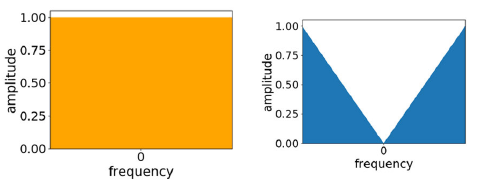
\includegraphics[width=0.5\textwidth]{Bachelorthesis/UsedImages/fig6.png}
    \caption{Rectangular Window (left) and Ram-Lak Filter (right)}
    \label{fig6}
\end{figure}
To reduce the influence of noise, especially in the higher frequency bands, various window functions are commonly applied. These act as regularizers by gradually rolling off or attenuating high-frequency components. Below, several standard choices are discussed.

\paragraph{Hamming Window}
The Hamming window introduces a smooth taper of the frequency response, which reduces the oscillations caused by abrupt cutoffs while still retaining a good portion of the lower and mid-frequency content. The functional form is given by
\[
w_\alpha(\omega) = (1-\alpha) + \alpha \cos\left(\frac{\pi \omega}{2 \Delta \omega K}\right), 
\quad K \in \mathbb Z,
\]
with a common parameter choice $\alpha = 0.46$. The resulting filter (figure~\ref{fig7}) acts approximately as a low-pass filter: it enhances low-frequency content, attenuates the high-frequency tail, and provides smoother transitions that reduce ringing artifacts in the reconstructed image. The Hamming filter is thus a good compromise between noise suppression and edge preservation.

\begin{figure}[h!]
    \centering
    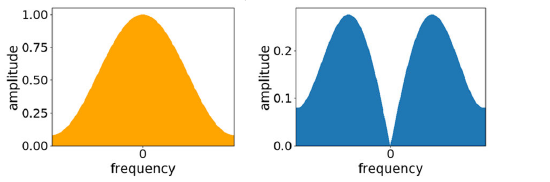
\includegraphics[width=0.5\linewidth]{Bachelorthesis//UsedImages/fig7.png}
    \caption{Hamming Window (left) and Hamming Filter (right)}
    \label{fig7}
\end{figure}

\paragraph{Hann Window}
The Hann window is closely related to the Hamming window, but with a different balance between the main lobe and side lobes. It is defined as
\[
w_\alpha(\omega) = (1-\alpha) + \alpha \cos\left(\frac{\pi \omega}{2 \Delta \omega K}\right), 
\quad K \in \mathbb Z,
\]
with the typical choice $\alpha = 0.5$. This parameterization results in a filter with stronger suppression of high frequencies compared to the Hamming window, leading to improved noise reduction at the cost of slightly more blurring in the reconstructed images. Figure~\ref{fig8} shows the Hann window and its resulting filter. The Hann filter is frequently chosen in practice when robustness to measurement noise is prioritized.

\begin{figure}[h!]
    \centering
    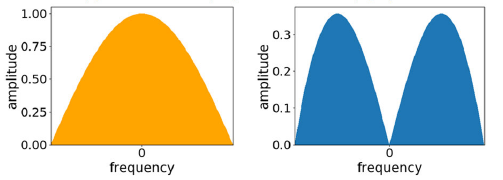
\includegraphics[width=0.5\linewidth]{Bachelorthesis/UsedImages/fig8.png}
    \caption{Hann Window (left) and Hann Filter (right)}
    \label{fig8}
\end{figure}

\paragraph{Cosine Window}
The cosine window is an alternative tapering strategy with a functional form
\[
w_\alpha (\omega) = \cos\left(\alpha \frac{\pi \omega}{2 \Delta \omega K}\right), 
\quad K \in \mathbb Z,
\]
where $\alpha = 1$ is a standard choice. Unlike the Hamming or Hann windows, the cosine window directly applies a cosine-based decay, resulting in a gradual but consistent suppression of frequencies as $\omega$ increases. As shown in figure~\ref{fig9}, the cosine window produces a smoother roll-off of high-frequency components, effectively reducing noise amplification while still allowing for relatively sharp image features. This window function is often selected when a balance between smoothness and detail preservation is desired.

\begin{figure}[h!]
    \centering
    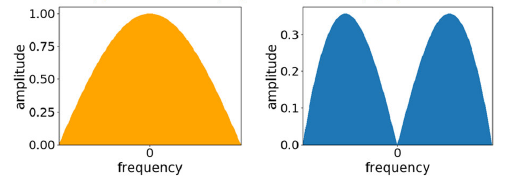
\includegraphics[width=0.5\linewidth]{Bachelorthesis/UsedImages/fig9.png}
    \caption{Cosine Window (left) and Cosine Filter (right)}
    \label{fig9}
\end{figure}

Although these smooth window functions are more robust to noises and ringing artifacts,
they reduce the image resolution by introducing a blurring effect (\cite{DeepFBP_CT}).

\section{Radiation dose in CT}

When performing a CT scan with the goal of image reconstruction, we are interested in high quality sinogram data. Since the Moore-Penrose inverse of $\mathcal R$ is discontinuous, even on our considered space $L_R^2$ , even small distortures in the projection data will result in remarkable errors in the reconstructed image~\cite{math_of_ct_wald}. We already introduce a degree of error due to discretizing the projection data, reconstructing the image on a finite amount of countable pixels and using interpolation to access non-available data for the backprojection step, hence additional noise and artifacts in the sinogram may make the reconstructed image to have even more distortures. With high quality CT imaging, patients can benefit from a quicker and more accurate diagnosis and precise anatomic information for planning therapeutic procedures. However the quality of the sinogram data and hence the of the reconstructed image depends on the initial radiation dose of the X-rays being shot through the patient, while the scan~\cite{Solomon_Marin_Choudhury_Patel_Samei_2017}. The physical processes, leading to the generation of X-rays are probabilistic, since they depend on collisions and quantum effects. 
\newline\newline
Inside a CT tube electrons are accelerated from cathode to the anode. The space between cathode and anode is vacuum, so electrons can travel freely. At this moment, each electron has a well-defined kinetic energy, but the randomness happens, once they hit the anode. There are four main possibilities. An elastic collision may occur, meaning, that the electron simply bounces from the anode and changes its traveling direction, leading to a little energy loss. Now an inelastic collision with the anode atom, tungsten, can have the outcome of X-ray production in 2 ways or can simply end up in the electron being slowed down and translating it's kinetic energy to heat. The characteristic X-ray production occurs, when a high-energy electron hits a tungsten atom and knocks out an inner shell electron, bringing the atom in an unstable state, an outer-shell electron falls into the vacancy to restore the stability of the atom, while the energy difference between the outer and inner shell is released as an X-ray photon. The breaking radiation occurs, when the high-speed electrons pass near the nucleus of a tungsten atom, now the positively charged nucleus attracts the electron, causing it to slow down and change the direction, so that the lost kinetic energy of the electron is emitted as an X-ray photon. It’s not predictable which outcome will occur for a single electron, because it depends on the electron’s kinetic energy, the quantum state of the tungsten atom, and other quantum-mechanical factors. When billions of electrons per second are accelerated to the anode, as in a CT scan, a stochastic model can be used to describe which outcomes are more likely. In general, most electrons lose their energy as heat, but if the electron has sufficient kinetic energy and interacts in the right way, it can produce X-rays either via bremsstrahlung or characteristic emission~\cite{Bushberg2021Ch2}.
\newline\newline 
The tube voltage (kVp) determines the energy of the electrons, in other words higher tube voltage results in electrons hitting the tungsten with higher energy, making the outcome of X-ray production higher per electron, while the tube current (mA) controls the number of electrons accelerated per second: a higher current leads to more electron–anode interactions and thus more photons overall, provided the tube voltage is sufficient to generate X-rays. 
\newline\newline
Now  X-ray photons are emitted in a random direction, but the anode geometry and collimators guide most of them toward the patient. As it passes through the tissue, the photon can transmit unimpeded and reach the detector, be absorbed by the tissue, if the photon itself has not sufficient initial intensity or scatter and change its traveling direction possibly missing the detector. This introduces another uncertainty, based on multiple factors, like particles on the way of the photon, since a common CT scan is not done in vacuum or the low intensity X-ray photon, because of the previous stochastic process and other quantum-mechanical properties, making it impossible to predict, what will happen to exactly what photon. High amount of emitted X-rays with high energy results in higher detection probability, speaking for the completeness of the sinogram data~\cite{Seibert_2004}.

\subsection{Consequences of high radiation dose}
While high image quality lies in patient's interest, since a precise diagnose may save his life and speed up the treatment, high dose CT may introduce negative consequences for a patient. The most important risk, is the increase in the stochastic effects, meaning, that radiation can damage DNA and cause mutations, that may lead to cancer in the long term. The probability of such effects rises with the patient dose. Deterministic effects occur when a sufficiently large number of cells in a tissue are damaged or killed, so that the tissue as a whole can no longer maintain its normal function. For such effects, a threshold dose exists: below this threshold, the tissue damage is too limited to cause any clinical symptoms, while above it, the severity of the effect increases with dose. However, the threshold is not a single exact value for every person but rather a statistical range, since individual radiosensitivity depends on factors such as genetics, age, health status, and previous radiation exposure. In diagnostic CT imaging, the absorbed doses are far below these threshold ranges, so deterministic effects do not occur. In interventional CT procedures, however, where the same area may be scanned repeatedly during needle guidance or treatment, localized doses can become high enough that deterministic effects like skin reddening, hair loss, or tissue necrosis may appear. Certain groups of patients are especially vulnerable to radiation: children are at higher risk because their tissues divide faster and they have a longer lifetime for possible effects to manifest; pregnant women and the fetus, particularly in the first trimester, are highly sensitive to radiation, with risks of malformations or later childhood cancers; young adults also carry higher lifetime risks compared to elderly patients. Additionally, patients who need repeated CT scans for chronic or oncological diseases accumulate dose over time, which further increases their overall risk. Finally, individuals with genetic predispositions that impair DNA repair mechanisms are more radiosensitive. For all these reasons, minimizing dose while preserving diagnostic quality is a central principle in CT imaging. For that reasons, a central area of research lies in improving the quality of reconstructed CT images with low dose CT to prevent such risks or at least to reduce the probability of the happenings through the scan itself~\cite{Bos2023RadiationExposureCT}.





\section{Statistics of the measurements}
\label{imageartifacts}
While filtered backprojection presents an implementation for the analytic approach to solve the image reconstruction task, there are iterative reconstruction algorithms, like the Algebraic Reconstruction Technique (ART) and Simultaneous Algberaic Reconstruction Technique (SART), modelling the reconstruction problem as a system of linear equations, representing the relationship between the image and its projections, iteraitvely updating the image to minimize discrepancies with the measured projections. These methods can handle incomplete data and reduce artifacts generally better, than the FBP pipeline, sincethey explicitely try to minimize the error, considering the noisy and incomplete data, while the FBP works with the assumption of complete, in best case continuous projection data. More advanced statistical iterative reconstruction (SIR) techniques explicitly account for the stochastic nature of X-ray photon detection. By incorporating noise models, SIR methods achieve improved image quality, especially in low-dose scans. Model-based iterative reconstruction (MBIR) extends this concept further by modelling the full physics of the CT system, including beam spectrum, detector response, scatter, combined with sophisticated regularization techniques. More recently, deep learning-based reconstruction has emerged as a powerful alternative, either by denoising and improving the image quality as a post-processing mechanism, after applying named reconstruction algorithms, even FBP. Despite the superior performance of iterative and model-based algorithms, FBP remains an area of interest. Its computational speed and simplicity make it crucial for real-time imaging. This section will give an explanation of some main sources of incomplete data.

\subsection{PCD measurements}
CT detectors are designed to convert incoming X-ray photons into a measurable electrical signal. There are two main types of detectors. Energy-integrating detectors (EIDs), being most common in clinical CT and photon-counting detetors (PCDs), offering a newer technology by counting individual photons. Unlike conventional energy-integrating detectors, which sum all photon energies over time, photon-counting detectors measure each arrived X-ray photon individually. PCDs are made of direct-conversion semiconductor materials~\cite{pcd_detec_paper}.
\newline\newline
An arriving X-ray photon interacts with the semiconductor atoms via photoelectric absorption or Compton scattering, depending on photon energy. In case of photoelectric absorption, it collides with a bound electron, usually in an inner shell. The photon transfers all its energy to the electron, ejecting it from the atom and making the atom ionized. In case of Compton scattering, a photon transfers only a part of its energy to a loosely bound (essentially free)  electron, unlike in the photoelectric absorption, where the energetic transfer happens to a bound electron and the photon is destroyed. In both cases, the electron is ejected, also called photoelectron. Now the scattered photon may escape or undergo further interactions, like another Compton scatter or photoelectric absorption. The ejected energetic photoelectron moves through the semiconductor lattice and excites electrons on its way, creating electron-hole pairs. Under an applied electric field, electrons and holes drift to electrodes (inside the detector), generating a measurable current pulse.  The magnitude of the current pulse is proportional to the energy deposited by the photon, because the number of electron-hole pairs and consequently the strength of the current pulse of the electric field depends on the photon energy. This shows, that too high tube voltage (kVp) will not improve the image quality anymore, because generated photons with too high energy will then more likely end up in Compton scattering, giving multiple, but partial signals, appearing as lower energy events, worsening energy resolution, ending with lack of contrast in the image.  The detector electronics compare the height of each current pulse against one or more predefined energy thresholds. Each time a pulse exceeds a threshold, it is registered as a photon detection. The number of such events in a time window gives the photon count $N(\theta, s)$. Performing an empty scan, gives the opprtunity to measure the mean number of arrived photons $N_0 (\theta, s)$ without patient's influence.
\newline\newline
In the first sections, the Beer–Lambert law was derived from the ratio of transmitted to incident intensities. In the case of photon-counting detectors, however, the detector output is not a direct measure of intensity but of the mean number of detected photons. Since the photon count is proportional to the photon flux, and hence to the beam intensity for a given energy spectrum and detector efficiency, the ratio of photon counts with and without the object approximates the corresponding intensity ratio (Taguchi et al., 2011; Persson et al., 2018). Thus, for the formation of the sinogram, the measured data are expressed as
\begin{equation}
    \frac{N(\theta, s)}{N_0(\theta, s)} \approx \frac{I(\theta, s)}{I_0(\theta, s)}.
\end{equation}
% \subsection{From PCD measurements to sinogram data}
% As discussed in the last subsection, the PCDs measure the photon count. In pracitice, both of these numbers are used to represent the sinogram data and not directly the intensity values, as defined earlier. This section aims to deliver some reasoning of such an approximation.
% \newline\newline
% We concentrate at some particular X-ray beam, at the line $L(\theta, s)$ for some $(\theta, s) \in [0, \pi) \times \mathbb R$, then $\Phi_0 (E)$, describes the \textit{incident spectral photon flux} (photons per unit area per unit time per unit energy) in $\frac{\mathrm{photons}}{s \cdot m^2 \cdot \mathrm{keV}}$. Analogousely, $\Phi(E)$ is the \textit{transmitted spectral photon flux}, after passing through the object, where $E$ is the photon energy. In the previous chapters, the attenuation coefficients of the object, we're interested in, depend only on the position $\textbf{x}$, but indeed, they also depend on the energy $E$, so that we obtain $f(E, \textbf{x})$, the \textit{linear attenuation coefficient} at energy $E$ and position $\textbf{x} \in \mathbb R^2$. In order to include the uncertainty of the detector, $\eta(E) \in [0,1]$ describes the \textit{detector quantum efficiency}, in other words, the probability, that a photon of energy $E$ is indeed counted by the detector. With $T$, we denote the \textit{exposure time}, so that $N_0$ is the \textit{expected (mean) number of counts} in $T$ with \textit{no object} present and $N$ is the \textit{expected (mean) number of counts} in $T$ with  the \textit{object}
\subsection{Quantum noise}

Suppose a detector measures the number of photons \(N\) along a ray $L(\theta, s)$ in a time interval of length \(T\), for \((\theta, s) \in [0, \pi) \times \mathbb{R}\). We split the interval \(T\) into \(n\) equal subintervals of length \(\Delta t = \frac{T}{n}\), with \(n \in \mathbb{N}\) and \(n > N\). Assuming independent photon arrivals at a constant average rate \(\mu = \frac{N}{T}\) photons per unit time, the probability of one photon arrival in a subinterval is
\[
p = \mu \cdot \Delta t = \frac{N}{n}.
\]

Then, the probability of no photon arrival is \(1-p\). Each subinterval is now a Bernoulli trial with outcomes: 1 photon with probability \(p\), or 0 photons with probability \(1-p\). Over \(n\) subintervals, the total photon count \(\tilde N\) follows a binomial distribution:
\[
P_n(\tilde N = k) = \binom{n}{k} p^k (1-p)^{n-k}.
\]

We now take the limit \(n \to \infty\) while keeping \(N\) constant~\cite{Chamberlain2016Poisson}:

\[
\begin{aligned}
P(\tilde N = k) 
&= \lim_{n \to \infty} \binom{n}{k} \left(\frac{N}{n}\right)^k \left(1 - \frac{N}{n}\right)^{n-k} \\[2mm]
&= \lim_{n \to \infty} \frac{n!}{k!(n-k)!} \left(\frac{N}{n}\right)^k \left(1 - \frac{N}{n}\right)^{n} \left(1 - \frac{N}{n}\right)^{-k} \\[1mm]
&= \lim_{n \to \infty} \frac{n(n-1)\cdots(n-k+1)}{k!} \frac{N^k}{n^k} \left(1 - \frac{N}{n}\right)^n \left(1 - \frac{N}{n}\right)^{-k} \\[1mm]
&= \frac{N^k}{k!} \lim_{n \to \infty} \left( \frac{n(n-1)\cdots(n-k+1)}{n^k} \right) \left(1 - \frac{N}{n}\right)^n \left(1 - \frac{N}{n}\right)^{-k} \\[1mm]
&= \frac{N^k}{k!} \cdot 1 \cdot e^{-N} \cdot 1 \\[1mm]
&= \frac{N^k e^{-N}}{k!}.
\end{aligned}
\]

Hence, in the limit, the total photon count \(\tilde N\) follows a Poisson distribution with mean \(N\):
\[
\tilde N \sim \mathrm{Poisson}(N).
\]

Therefore, the measured photon count \(\tilde{N}(\theta, s)\) including attenuation by the object can be modeled as
\[
\tilde{N}(\theta, s) \sim \mathrm{Poisson}\Big(N_0(\theta, s) \exp\Big(-\int_{L(\theta, s)} f(x,y) \mathrm{d}L \Big)\Big),
\]
where \(N_0(\theta, s)\) is the expected number of photons without the object and \(f(x,y)\) is the object's attenuation coefficient. This captures the quantum noise inherent in photon-counting CT measurements.

\subsection{Electronic noise}
The last subsection examined the source of the noise, which is present, even in measurements with detectors, capturing every photon count perfectly. The electronic noise represents the second main source of noise, present in the measurements, caused by the detection system itself.
\newline\newline
In modern CT systems, electronic noise usually has a negligible effect for protocols, using typical dose levels and for normal-size patients, but for low-dose protocols or obese patients, electronic noise becomes more important because the detected signal may become comparable to the electronic noise level. This noise originates from
physical processes within the detector system and its associated electronics and is independent of the number of detected photons. Unlike quantum noise, which follows a
Poisson distribution, electronic noise is typically modeled as Gaussian with zero mean and constant variance, adding more uncertainty to the sinogram data, worsening and image quality
after the reconstruction in low dose CT~\cite{Xie2017Robust}.
\begin{equation}
    \varepsilon \sim \mathcal N(0, \sigma^2).
\end{equation}
Now the entire photon counting procedure can be modelled as the sum of both distributions, so that for $(\theta, s) \in [0, \pi) \times \mathbb R$
\begin{equation}
    \tilde N(\theta, s) \sim \mathrm{Poisson}(N_0 \exp(-\int_{L(\theta, s)} f(\textbf{x}) \mathrm{d} \textbf{x})) + \mathcal{N}(0, \sigma^2)
\end{equation}

\section{Image quality problem of low dose CT}
Lowering the radiation dose in CT, typically achieved by reducing the tube current or the exposure time, directly reduces the expected number of photons \(N\) reaching the detector. While this reduction is beneficial for patient safety, it has direct consequences on the image quality.  
\newline\newline
To quantify the impact, it is useful to consider the \emph{relative noise}, defined as the standard deviation of the measurement divided by its mean. In 
\[
\text{Relative noise} = \frac{\sqrt{N+ \sigma^2}}{N} \propto \frac{1}{\sqrt{N}}.
\]
This indicates that as \(N\) decreases, the relative fluctuations increase. In other words, the lower the dose, the higher the statistical uncertainty in each measurement~\cite{Xie2017Robust}.  


\section{Image noise suppression, using FBP}

There are three main different approaches to suppress image noise, using the FBP reconstruction, ew. One of them operates in the sinogram domain, aiming to preprocess the data before the FBP reconstruction. The second opportunity deals with improvements within the FBP pipeline itself and the third most common way works as a post-processing method, trying to supress the noise directly in the image space after the FBP reconstruction. 

\subsection{Sinogram preprocessing}
As mentioned in the last section, the increase of relative fluctuations in sinogram data of low-dose CT is natural. To address the issue of quantum and electronic noise, many CT sinogram recovery methods (CTSR) haven been proposed, in order to estimate the ideal ones from the acquired noisy sinograms and then reconstruct the final high-quality CT image from the estimated ideal sinogram. They can be categroized into two main classes: the post-log and pre-log methods. The post-log CTSR methods restore the sinograms usually, using statistical iterative algorithms, in particular by assuming the mixed noise in the measured sinogram data as Gaussian, a penalized weighted (PWLS) function is typically used. Although PWLS possesses the advantage of easy computation attributed to its weighted least-square form, it fails to accurately use the Poisson-distribution-characteristic underlying the pre-log projection data. Specifically, the logarithm operation on projection data can result in amplification of the noise, especially for low-dose CT imaging. On the other hand, the pre-log CTSR methods use the Beer-Lambert law to construct the forward model and directly recover pre-log projection data from the Poisson-distribution-assumption of the measurements. With appropriate statistical models, the pre-log CTSR regime can accommodate the non-positive values in the measurements. To further model electronic noise, the shifted Poisson and the Gaussian models in the pre-log domain have also been adopted. However, these methods still consider the electronic noise background in a heuristically approximate way and do not fully inject the intrinsic statistical “Poisson+Gaussian” properties~\cite{Xie2017Robust}. 
\newline\newline
Both of the methodologies operate, using a Maximum a posteriori (MAP) framework, minimizing an objective function iteratively for a given sample, motivating the idea to scale the idea on an entire dataset, using a neural network. Recently, the fast development of convolutional neural network (CNN) based deep learning (DL) techniques have expedited many successful applications in the field of medical imaging. DL techniques can efficiently exploit high-level features from the pixel level through a hierarchical multilayer framework. In the work by Yin et al.~\cite{Yin2021}, a domain progressive 3D residual convolution network was used. The DP-ResNet consists of three main parts: sinogram domain sub-network (SD-net), FBP and image domain-subnetwork (ID-net). The paper introduces 3 different strategies, where separately the usage of the SD-net, of the ID-net and the simultaneous integration (DP-ResNet) were examined. The results from the table ... show, that the sinogram domain learning, using a neural network delivers better results, than vanilla FBP for low dose CT.
\subsection{Modifications within FBP}
The second class of methods targets the FBP pipeline itself, aiming to improve the filtering or backprojection stages. Filtering in the projection domain is one of the most important operations in FBP, in which a classical window function, such as the Rectangular window, the Hamming window, the Hann window, the Cosine window, or the Sine window is manually selected for the reconstruction. Sophisticated window function has also been developed and shown improved performance in CT reconstruction.
For example, Yu et al. applied the Parzen window in the
filtered back-projection algorithm~\cite{DeepFBP_CT}. Modified window functions were also developed, to achieve balance between noise suppression and resolution preservation~\cite{DeepFBP_CT}. Different from existing studies, Xi Tan, et all.~\cite{DeepFBP_CT}, designed a neural network to implicitly learn an optimized window function for the FBP, showing a good performance of low-dose reconstructions, without introducing a burden of computational complexity (after the learning). 
\newline\newline
The interpolation operator during the back-projection plays an important role in FBP~\cite{DeepFBP_CT}. The linear interpolation is a popular selection in the traditional FBP algorithm. Note that linear interpolation is vulnerable to noise, and may lead to information loss in the process of back-projection. Different interpolation methods have been proposed for FBP. Horbelt et al. considered using spline interpolation to improve the standard FBP reconstruction. Schaller et al. presented a spiral interpolation approach for multislice spiral computed tomography. An interpolation operator was introduced, using neural networks~\cite{DeepFBP_CT}. This new interpolation method can utilize more information from nearby detector bins. The results from ... show, that the integration of neural networks within the analytical FBP pipeline itself is able to provide noise suppression and better image quality in low-dose CT. 
\subsection{Image Post-Processing}
The third, most common class of methods targets the work with the produced image itself. The most popular way, is to use deep-learning as a post-processing procedure, that suppresses noise and artifacts in images, reconstructed by FBP. For example, Chen et al. used RED-CNN and Wu et al. used an improved DnCNN,
both to suppress noises on reconstructed CT images. Other
post-processing algorithms may use the perceptual loss, generative adversarial networks (GAN), and
multiple CT image layers information. Overall this strategy also enhances the final image quality of low-dose CT~\cite{DeepFBP_CT}.
\section{Methodology}
So far, we have described the basics of analytical image reconstruction in CT and explained in detail the main problem of the commonly used reconstruction algorithm, especially with regard to low-dose CT, which aims to protect the health of the patient, followed by state-of-the-art methods that aim to improve the reconstruction quality when using noisy projection data. This section aims to present the methodology of this work, to suppress the image noise of low-dose CT, involving the FBP algorithm and different neural network applications.

\subsection{LoDoPaB}
Deep Learning based approaches benefit strongly from the availability of comprehensive datasets, which are unfortunately rarely available~\cite{leuschner2022lodopab}. Comparing different learned methods is a challenging task, especially when referring to CT reconstructions, since they are highly bounded to the used dataset and setup for training. To this end, Johannes Leuschner et al.~\cite{leuschner2022lodopab} introduced the Low-Dose Parallel Beam (LoDoPaB)-CT dataset,  based on the public LIDC/IDRI database of human chest CT reconstructions. These are used as 2D images, to represent the ground truth. The projections are created, by simulating low photon count CT measurements with a parallel beam scan geometry. Such paired samples construct the most complete training data and could be used for all kinds of learning. In total, the dataset features more than 40000
sample pairs from over 800 different patients

\subsubsection{Ground truth data extraction process}
The data generation process starts with the extraction of the ground truth reconstructions from the LIDC/IDRI dataset, which represent high quality CT images. The images are first cropped to the central rectangle of $362 \times 362$ pixels, because most of the images contain (approximately) circle-shaped reconstructions with a diameter of $512$ pixels. After cropping, the image contains the pixel values, lying inside the circle, avoiding value jumps, occurring at the border of the circle, yielding the ground truth images, which only show some interior part of the objects.
\newline\newline
In the next step, the pixel values of the images are transformed into integer Hounsfield unit (HU), used to express CT density. Now a uniform noise from the interval $[0,1)$ is added, to transform the discrete distribution of the stored values into a continuous distribution, which is a common assumtpion of image modells. Now the linear attenuation coefficients are computed from dequantised HU values, using the common definition of HU and the linear attenuation coefficients $\mu_\mathrm{water} = 20m^{-1}, \mu_\mathrm{air} = 0.02m^{-1}$~\cite{leuschner2022lodopab}.
\begin{equation}
    \mathrm{HU} = 1000 \frac{\mu - \mu_\mathrm{air}}{\mu_\mathrm{water} - \mu_\mathrm{air}} \qquad \Leftrightarrow \qquad \mu = \mathrm{HU} \frac{\mu_\mathrm{water} - \mu_\mathrm{air}}{1000} + \mu_\mathrm{water}
\end{equation}
In the final step of the ground truth extraction process, the $\mu$-values are normalised into $[0,1]$ by the division by 
\begin{equation}
    \mu_\mathrm{max} = 3071 \frac{\mu_\mathrm{water} - \mu_\mathrm{air}}{1000} + \mu_\mathrm{water} = 81.35858 m^{-1},
\end{equation}
corresponding to the largest HU value, that can be represented with the standard 12-bit encoding, ie. $(2^{12} - 1 - 1024) \mathrm{HU} = 3071\mathrm{HU}$, followed by a clip into $[0,1]$. The whole ground truth extraction procedure is summarized in the following pseudocode.

\begin{algorithm}
\caption{Ground Truth Extraction}\label{alg:gt_ext}
\begin{algorithmic}[1] % The [1] enables line numbers
\Require An image $z$ from the LIDC dataset
\Ensure Ground Truth Image for LoDoPaB dataset 

\State $\overline{z} \gets \mathrm{\textbf{center\_crop}(z, 362 \times 362)}$
\State $\mathrm{image\_hu \gets \textbf{pixels\_to\_HU}(\overline{z})}$
\State $\mathrm{image\_hu \gets image\_hu + noise}$
\State $\mathrm{image\_mu} \gets \mathrm{image\_hu \cdot (\mu_{water} - \mu_{air})/1000 + \mu_{water}}$
\State \Return $\mathrm{\textbf{clamp}(image\_mu/\mu_{max}, 0, 1)}$
\end{algorithmic}
\end{algorithm}

\subsubsection{Low dose projection data generation process}
The last subsection explained the way, ground truth data is being extracted for the LoDoPaB dataset. Now is the goal to simulate low-dose CT projection data. In order to avoid the same geometries of the forward operation, a higher resolution for the simulation was used. They used bilinear interpolation, to scale the ground truth from $362 \times 362$ to $1000 \times 1000$ pixels. Now the non-normalised, upscaled image is projected by the ray transform, to get to the projection data $\mathcal R f$. Here, $513$ equidistant detector bins were assumed, spinning the image diameter on a domain size of $26 \times 26$ centimeters and $1000$ equidisitant angles between $0$ and $\pi$. Based on this projection data, the measured photon counts $\tilde N_1$ are sampled, while generated Poisson noise is added, so that 
\begin{equation}
    \tilde N_1 \sim \mathrm{Poisson}(N_0 \cdot \exp(-\mathcal R f))
\end{equation}The sampling in some cases yields photon counts of zero, which we then replace by photon counts of 0.1. Hereby strictly positive values are ensured, which is a pre-requisite for the log-transform in the next step. Now the negative logarithm of the photon counts quotient,  $-\frac{\max(0.1, \tilde N_1)}{N_0}$ is taken, resulting in the post-log measurements, finally divided by $\mu_\mathrm{max}$, to match the normalized ground truth images. Below is the summary of the steps of the projection data generation process. 
\begin{algorithm}
\caption{Low dose sinogram data generation}\label{alg:ld_gen}
\begin{algorithmic}[1] % The [1] enables line numbers
\Require A ground truth image $x$, ensured from algorithm~\ref{alg:gt_ext}
\Ensure Simulated low dose sinogram data 

\State $\overline{x} \gets \mathrm{\textbf{bilinear\_interpolation}(\mu_{max}} \cdot x, 1000 \times 1000)$
\State $y \gets \mathrm{\textbf{RadonTransform}}(\overline{x}, \mathrm{angles: 1000}, \mathrm{detectors: 513} )$
\State $\mathrm{photons} \gets \max(\mathrm{Poisson}(\exp(-y) \cdot 4096, 0.1)$
\State \Return $-\log(\mathrm{photons}/4096)/\mu_{\mathrm{max}}$
\end{algorithmic}
\end{algorithm}

\subsection{Evaluation metrics}

To evaluate the image quality, the PSNR (peak signal-to-noise ratio) is used as an evaluation metric, to quantify the reconstruction quality with respect to inexact approximations (e.g. sensitivity to blurry details), where higher PSNR values (in dB) indicate less error between reconstructed image and ground truth image~\cite{DeepFBP_CT}. SSIM (Structural similarity index measure) is used to measure the similarity in the structure between the reconstructed image and the ground truth image, where higher value also indicates higher similarity~\cite{DeepFBP_CT}. The $L_2$-Loss emphasizes large errors and is sensitive to overall pixel precision, making it effective for detecting strong distortions, while the $L_1$, on the other hand, is more robust to the outliers and better preserves edge details, than $L_2$

\subsection{Window function as an optimizable vector only}
The window function, used as a common regularization technique in the FBP algorithm plays an important role for the reconstruction quality, as mentioned in section~\ref{281}. In~\cite{DeepFBP_CT}, the learnable filter in the frequency domain is directly defined as the optimizable vector, proposing two learning strategies.
\newline\newline
The first opportunity suggests, to keep the dependency on detector positions only and so to use the same filter for every projection angle between $0$ and $\pi$. Initializing the window vector with ones and learning the 513 components, is the procedure, being applied in~\cite{DeepFBP_CT}. The second strategy uses more parameters by introducing the angle dependency, creating the opportunity to learn $1000 \times 513$ components.
\newline\newline
Strategy II delivered better image quality, than Strategy I, trained with same conditions, making it reasonable to build on that. The first idea is to disable the post processing network and to use linear interpolation, as in the standard FBP pipeline~\cite{DeepFBP_CT}, to observe whether the optimizable window vector is capable to suppress the image noise, being caused by the simulated low-dose sinogram data, leading to the setup, visualized in figure~\ref{fig:experiment1_setup}.
\begin{figure}[h!]
    \centering
    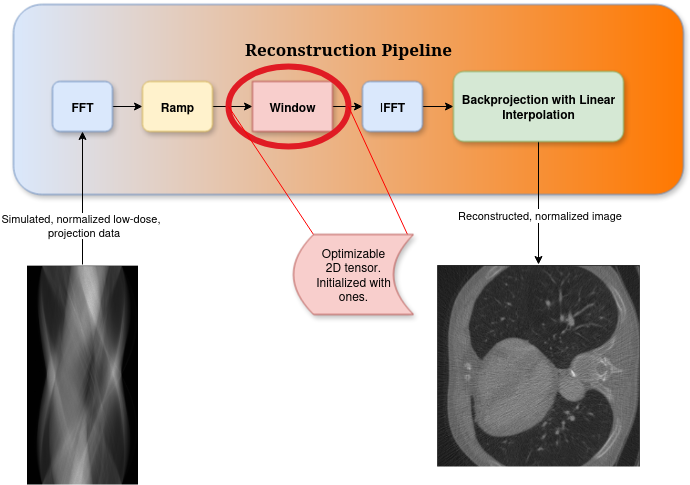
\includegraphics[width=0.8\textwidth]{Bachelorthesis//UsedImages/experiment1.png}
    \caption{The reconstruction setup, using the standard FBP algorithm with optimizable window function, as a vector}
    \label{fig:experiment1_setup}
\end{figure}

\subsubsection{Overfitting on 1 sample, using $L_2$ loss}

 Overfitting with 1 data sample, in order to see, whether the task is being understood, produced result, visable in figure~\ref{fig:windowII+l2+slow}. One can see in~\ref{fig:windowII+l2+slow50_loss}, that the loss function went consistently down, reached values under $10$ and was still going down after $3000$ iterations, showing, that the model learned something. From~\ref{fig:windowII+l2+slow50_images} is remarkable, that the model understood the main task of image quality enhancement and that the pixelwise loss was completely sufficient for 1 sample, to be able to reproduce the quality of the ground truth image, removing noise, gaining enough contrast and reproducing even small, but possibly very important details, showing the excellent (perceptual) reconstruction quality of the optimized window function, compared to other common regularizers, discussed in~\ref{281}.From~\ref{fig:windowII+l2+slow50_filters}, where the angular mean of the optimized filter is compared to the common filter choices, can be obtained, that the learned window function tends to suppress the high frequency components of the non-bounded ramp filter, showing the behavior of the common regularization methods, introduced in section~\ref{281}. \ref{fig:windowII+l2+slow50_windows} confirms the last observation by showing, that the optimized window function follows the slope of the Hann window, while still allowing a portion of the highest frequency components to participate, reflecting the behavior of the Hamming filter at the highest frequencies. Further, from \ref{fig:windowII+l2+slow50_windows} and \ref{fig:windowII+l2+slow50_filters}, strong jitter can be observed in the learned window function and consequentially in the learned filter, especially at the lowest frequencies, raising the question, whether it is caused by general training instability or because of the task of overfitting on 1 sample, the model trying to reproduce the original image. The try was successful, since the learned filter achieved outstanding metrics in compairson to the common regularizers \ref{fig:windowII+l2+slow50_metrics}.

 \begin{figure}[h!] % The [h!] option forces the figure to be placed "here" if possible.
    \centering % Centers the entire figure on the page.
    \newcommand\size{0.4}
    % --- The first subfigure ---
    \begin{subfigure}[t]{\size\textwidth}
        \centering
        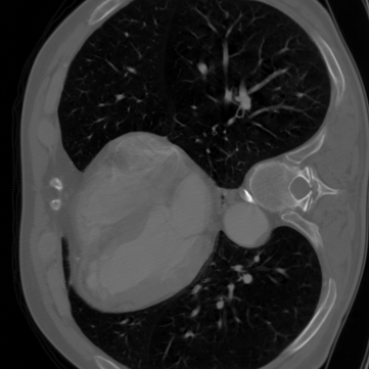
\includegraphics[width=\textwidth]{Bachelorthesis/UsedImages/gt_50.png}
        \caption{Ground-truth image} % You can add a sub-caption here if needed, e.g., \caption{Control Group}
        \label{fig:windowII+l2+slow50_gt}
    \end{subfigure}
    \hfill % This command adds stretching horizontal space between the two images.
    % --- The second subfigure ---
    \begin{subfigure}[t]{\size\textwidth}
        \centering
        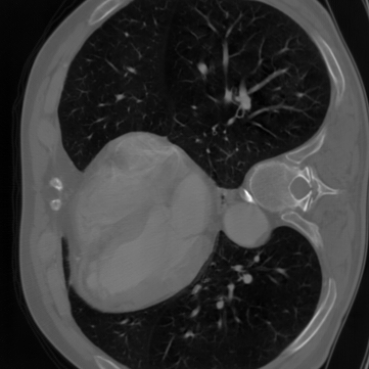
\includegraphics[width=\textwidth]{Bachelorthesis//UsedImages/l2_0.001_50_3000.png}
        \caption{\textbf{Reconstructed low-dose image, using FBP with the optimized filter}}
        \label{fig:windowII+l2+slow50_learned}
    \end{subfigure}
    \hfill
    \begin{subfigure}[t]{\size\textwidth}
        \centering
       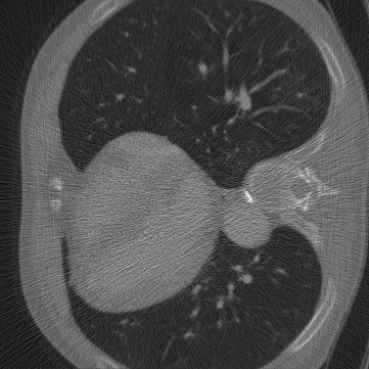
\includegraphics[width=\textwidth]{Bachelorthesis//UsedImages/vanilla_50.png}
        \caption{Reconstructed low-dose image, using vanilla FBP, from~\ref{practical_impl}}
        \label{fig:windowII+l2+slow50_vanilla}
    \end{subfigure}
     % Adds space between the second and third images.
    % --- The third subfigure ---
    \hfill
    \begin{subfigure}[t]{\size\textwidth}
        \centering
        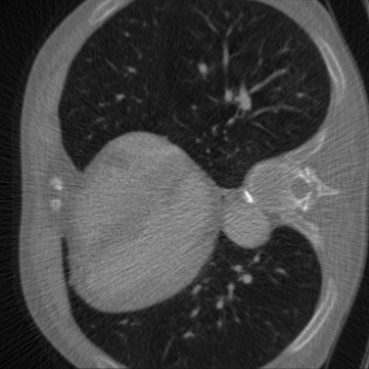
\includegraphics[width=\textwidth]{Bachelorthesis//UsedImages/hamming_50.png}
        \caption{Reconstructed low-dose image, using FBP with the hamming filter, from ~\ref{281}}
        \label{fig:windowII+l2+slow50_hamming}
    \end{subfigure}
    \hfill
    \begin{subfigure}[t]{\size\textwidth}
        \centering
        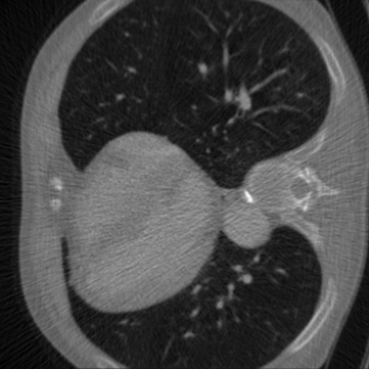
\includegraphics[width=\textwidth]{Bachelorthesis//UsedImages/hann_50.png}
        \caption{\textbf{Reconstructed low-dose image, using FBP with the hann filter, from ~\ref{281}}}
        \label{fig:windowII+l2+slow50_hann}
    \end{subfigure}
    \hfill
    \begin{subfigure}[t]{\size\textwidth}
        \centering
        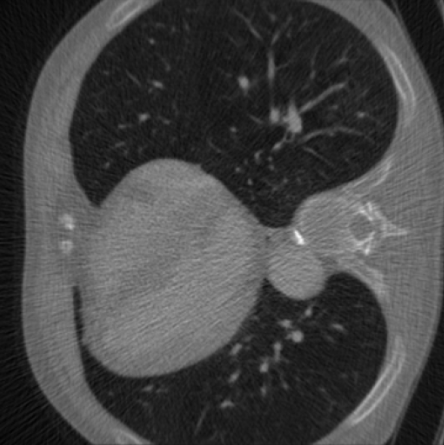
\includegraphics[width=\textwidth]{Bachelorthesis//UsedImages/cosine_50.png}
        \caption{Reconstructed low-dose image, using FBP with the cosine filter, from ~\ref{281}}
        \label{fig:windowII+l2+slow50_cosine}
    \end{subfigure}
        
    \caption{Image result of the overfitting procedure on 50-th sample from the training set, using $L_2$ loss as criterion with an initial learning rate of $0.001$, optimizing the window function.}
    \label{fig:windowII+l2+slow50_images} % A label for referencing the entire figure.
\end{figure}

\begin{figure}
    \centering
    \begin{subfigure}[t]{0.49\textwidth}
        \centering
        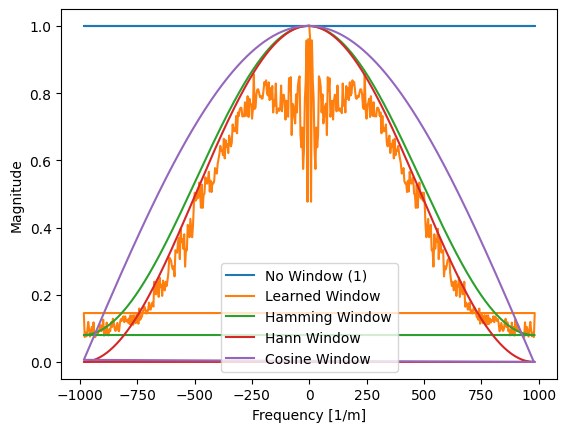
\includegraphics[width=\textwidth]{Bachelorthesis//UsedImages/exp1_window_function.png}
        \caption{Window compairson}
        \label{fig:windowII+l2+slow50_windows}
    \end{subfigure}
    \hfill
    \begin{subfigure}[t]{0.49\textwidth}
        \centering
        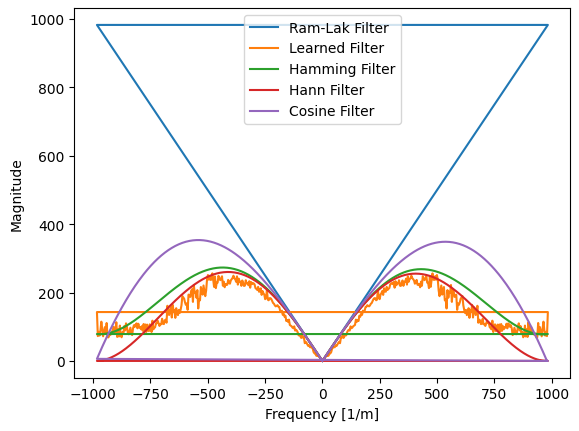
\includegraphics[width=\textwidth]{Bachelorthesis//UsedImages/exp1_filters.png}
        \caption{Filter compairson}
        \label{fig:windowII+l2+slow50_filters}
    \end{subfigure}
    \hfill
    \begin{subfigure}[t]{1\textwidth}
        \centering
        \begin{tabular}{lccccc}
        \toprule
        Method & PSNR (dB) & $L_2$ & MAE & MSE & SSIM \\
        \midrule
        Vanilla & 23.1395 & 636.0084 & 0.0568 & 0.0049 & 0.4547 \\
        \textbf{Learned filter}    & \textbf{42.5557} & \textbf{7.2740} & \textbf{0.0060} & \textbf{5.5508e-5} & \textbf{0.9810} \\
        Hamming filter & 25.2575 & 390.5404 & 0.0487 & 0.0030 &  0.5673 \\
        \textbf{Hann filter} & \textbf{25.3343} & \textbf{383.6972} & \textbf{0.0486} & \textbf{0.0029} & \textbf{0.5776} \\
        Cosine filter & 24.9264 & 421.4795 & 0.0496 & 0.0032 & 0.5362 \\
        \bottomrule
        \end{tabular}
        \caption{Quantitative comparison}
        \label{fig:windowII+l2+slow50_metrics}
    \end{subfigure}
    \hfill
    \begin{subfigure}[t]{0.49\textwidth}
        \centering
        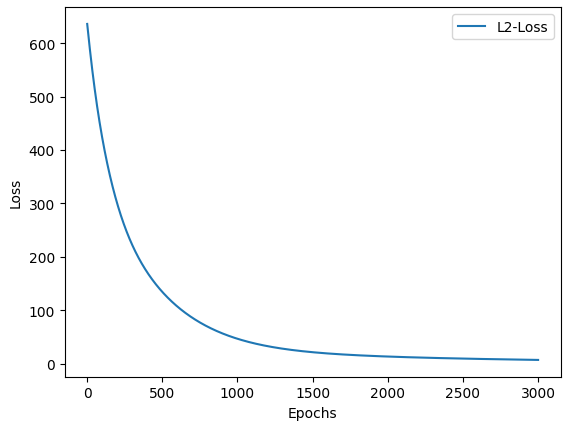
\includegraphics[width=\textwidth]{Bachelorthesis//UsedImages/l2_firstexp.png}
        \caption{The loss curve during overfitting}
         \label{fig:windowII+l2+slow50_loss}
    \end{subfigure}
    % --- The main caption for the entire figure ---
    \caption{Results of the overfitting procedure on 50-th sample from the training set, using $L_2$ loss as criterion with an initial learning rate of $0.001$, optimizing the window function.}
    \label{fig:windowII+l2+slow} % A label for referencing the entire figure.
\end{figure}
 \subsubsection{Training on a subset, using $L_2$ loss}
 The result from the last experiment motivates to extend the training setup. For that reasons, the setup from figure~\ref{fig:experiment1_setup} is now applied to a subset of LoDoPaB, containing 1000 samples. Since the initial learning rate of $0.001$ was totally sufficient for overfitting within $3000$ iterations without the intervention of the learning rate scheduler, the same initial learning rate was also used in this case. The training with the Adam optimizer and the $L_2$ loss was run for $100$ epochs, while the progress was tracked every $10$ epochs. In order to provide meaningful training results, the evaluated samples were taken in increments of $100$, since the images next to each other represent nearest patient slices. Before investigating the window performance on the validation dataset, the behavior on the training dataset is first observed, to examine, how the window function behaves on already seen data.
 \newline\newline
 After $10$ epochs of training, being equivalent to $10000$ iterations, the window function already shows some results. 

 \begin{figure}[h!] % The [h!] option forces the figure to be placed "here" if possible.
    \centering % Centers the entire figure on the page.
    \newcommand\size{0.49}
    % --- The first subfigure ---
    \begin{subfigure}[t]{\size\textwidth}
        \centering
        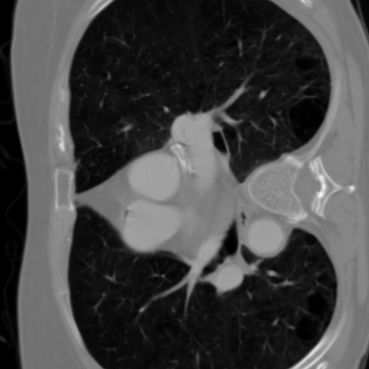
\includegraphics[width=\textwidth]{Bachelorthesis/UsedImages/Train1000_L2_100epochs/Training_L2_1000_100epochs_after10/gt_0_train1000l2100.png}
        \caption{Ground-truth image (1. sample)} % You can add a sub-caption here if needed, e.g., \caption{Control Group}
        \label{fig:windowII+l2+slow+subset_gt0}
    \end{subfigure}
    \hfill % This command adds stretching horizontal space between the two images.
    % --- The second subfigure ---
    \begin{subfigure}[t]{\size\textwidth}
        \centering
        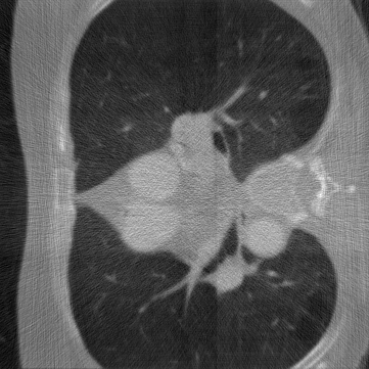
\includegraphics[width=\textwidth]{Bachelorthesis/UsedImages/Train1000_L2_100epochs/Training_L2_1000_100epochs_after10/pred_0_train1000l2100.png}
        \caption{\textbf{Predicted image (1. sample)}}
        \label{fig:windowII+l2+slow+subset_learned0}
    \end{subfigure}
    \hfill
    \begin{subfigure}[t]{\size\textwidth}
        \centering
       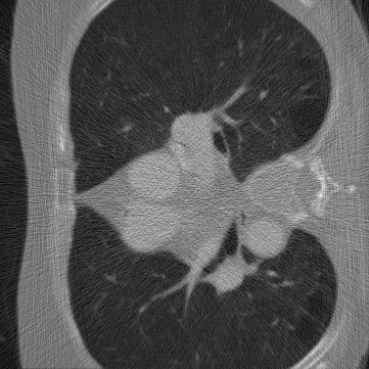
\includegraphics[width=\textwidth]{Bachelorthesis/UsedImages/Train1000_L2_100epochs/Training_L2_1000_100epochs_after10/vanilla_0_train1000l2100.png}
        \caption{Vanilla image (1. sample)}
        \label{fig:windowII+l2+slow+subset_vanilla0}
    \end{subfigure}
    \caption{Learning result of the 1. sample of the training dataset, after 10 epochs of training, using $L_2$ loss as criterion to minimize and an initial learning rate of $0.001$, optimizing the window function}
    \label{fig:windowII+l2+1000_image1} % A label for referencing the entire figure.
\end{figure}

\begin{figure}[h!]
    \centering % Centers the entire figure on the page.
        \newcommand\size{0.49}
    \begin{subfigure}[t]{\size\textwidth}
        \centering
        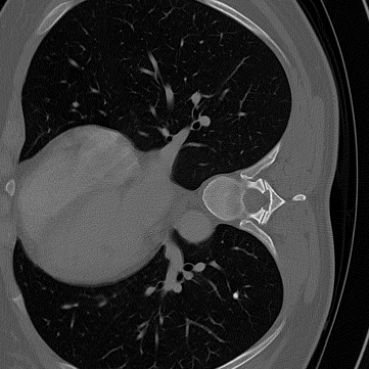
\includegraphics[width=\textwidth]{Bachelorthesis/UsedImages/Train1000_L2_100epochs/Training_L2_1000_100epochs_after10/gt_100_train1000l2100.png}
        \caption{Ground-truth image (100. sample)} % You can add a sub-caption here if needed, e.g., \caption{Control Group}
        \label{fig:windowII+l2+slow+subset_gt100}
    \end{subfigure}
    \hfill % This command adds stretching horizontal space between the two images.
    % --- The second subfigure ---
    \begin{subfigure}[t]{\size\textwidth}
        \centering
        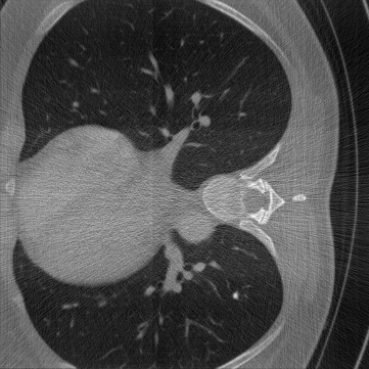
\includegraphics[width=\textwidth]{Bachelorthesis/UsedImages/Train1000_L2_100epochs/Training_L2_1000_100epochs_after10/pred_100_train1000l2100.png}
        \caption{\textbf{Predicted image (100. sample)}}
        \label{fig:windowII+l2+slow+subset_learned100}
    \end{subfigure}
    \hfill
    \begin{subfigure}[t]{\size\textwidth}
        \centering
       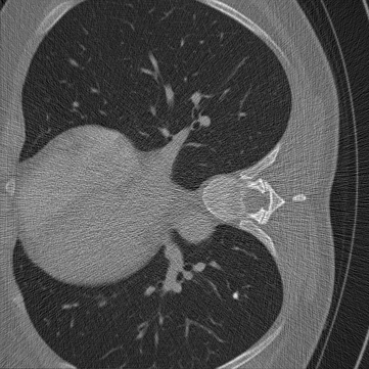
\includegraphics[width=\textwidth]{Bachelorthesis/UsedImages/Train1000_L2_100epochs/Training_L2_1000_100epochs_after10/vanilla_100_train1000l2100.png}
        \caption{Vanilla image (100. sample)}
        \label{fig:windowII+l2+slow+subset_vanilla100}
    \end{subfigure}
    \caption{Learning result of the 100. sample of the training dataset, after 10 epochs of training, using $L_2$ loss as criterion to minimize and an initial learning rate of $0.001$, optimizing the window function}
    \label{fig:windowII+l2+1000_image100} % A label for referencing the entire figure.
 \end{figure}

\section{Conclusion}
\section{Summary}
\section{Future work}

\bibliographystyle{plain}
\bibliography{Bachelorthesis/bibliography}  % filename without .bib extension
\end{document}
% Continue here with rest of mathematical derivation...

